\documentclass[12pt]{article}
\usepackage[utf8]{inputenc}
\usepackage[T2A]{fontenc}
\usepackage[russian]{babel}
\usepackage{amsmath}
\usepackage{amssymb}
\usepackage{dsfont}
\usepackage[dvipsnames]{xcolor}
\usepackage{setspace}
\usepackage{multirow}
\usepackage[a4paper, outer=1.5cm, inner=1.5cm, top=1cm, bottom=1cm]{geometry}
\usepackage{graphicx}
\usepackage{skull}
\usepackage{wasysym}
\usepackage{float}
\graphicspath{{.images/}}
\usepackage{hyperref}
\hypersetup{colorlinks=true, linkcolor=blue, filecolor=magenta, urlcolor=cyan}
\usepackage[firstpage]{draftwatermark}
\SetWatermarkText{
    $\qquad\qquad\qquad\qquad\qquad$\parbox{7cm}{\begin{center}
    
\includegraphics[width = 0.08\textwidth]{lion-logo.png}\bigskip\\~\bigskip\\~\vspace{-24mm}\\~\end{center}}
}
\SetWatermarkAngle{0}
\SetWatermarkScale{1.5}
\usepackage{etoolbox}

\newtoggle{ifsolved}
\newtoggle{needhelp}
\newcounter{num}
\setcounter{num}{1}

\newcommand{\newnum}{\par\textbf{\textnumero\arabic{num}}\stepcounter{num}}
\newcommand{\sol}{\vspace{3mm}\par\textbf{Решение: }}
\newcommand{\ans}{\vspace{3mm}\par\textbf{Ответ: }}
\newcommand{\hint}{\vspace{3mm}\par\textbf{Подсказка: }}
\newcommand{\mode}[1]{
\ifstrequal{#1}{0}{\togglefalse{ifsolved}\togglefalse{needhelp}}{\ifstrequal{#1}{1}{\togglefalse{ifsolved}\toggletrue{needhelp}}{\ifstrequal{#1}{2}{\toggletrue{ifsolved}\togglefalse{needhelp}}{\toggletrue{ifsolved}\toggletrue{needhelp}}}}} %if 0 - if 1 - if 2 - else
%\newenvironment{problem}[8]{%#1, #2, #3
%\parbox{\linewidth}{\vspace{4mm}\ifstrequal{#4}{(лёгкая)}{\newnum\textbf{.}}{\newnum\textbf{*.} } \\ #5}
%\iftoggle{ifsolved}{\sol #6}{}
%\iftoggle{ifsolved}{\ans #7}{}
%\iftoggle{needhelp}{\hint #8}{}}

\newenvironment{problem}[8]{%#1, #2, #3
\parbox{\linewidth}{\vspace{5mm}\ifstrequal{#4}{(лёгкая)}{\newnum\textbf{.}}{\newnum\textbf{*.} } \\ #5}
\iftoggle{ifsolved}{\sol #6}{}

\iftoggle{ifsolved}{\parbox{\linewidth}{\ans #7}}{}
\iftoggle{needhelp}{\parbox{\linewidth}{\hint #8}}{}}

\newenvironment{mylist} %custom list
{ \begin{itemize}
    \setlength{\itemsep}{0pt}
    \setlength{\parskip}{0pt}
    \setlength{\parsep}{0pt}     }
{ \end{itemize}                  }

\newenvironment{homeass}[1]{\vspace*{-1.5cm}
\iftoggle{ifsolved}{
    \section*{\center{Решение домашнего задания к #1.}}
}{
    \section*{\center{\textcolor{Sepia}{Домашнее задание к #1}}}
} \vspace{7mm}\large}

\parindent=0pt
\pagestyle{empty}
%$\!$[\arabic{class}.\arabic{num}]
%\ifnumcomp{\value{counter}}{>}{1}{true}{false}
%\definecolor{Gray}{gray}{0.9}
%\definecolor{mypink}{RGB}{219, 48, 122}
%\newcolumntype{g}{>{\columncolor{Gray}}p{2.8cm}}

\begin{document}
\large
\mode{7}
%0 for problems without hints
%1 for problems + hints
%2 for problems + solutions + answers
%else: show all

{\centering\section*{СПИСОК ЗАДАЧ}}

{\centering\subsection*{\smallskip\\\textcolor{green}{\textbf{Полезные вещи, которые можно и нужно копипастить:}}}}

\subsection*{\textcolor{Emerald}{\textbf{Полезные шпаргалки по LaTeXу:}}}

\textbf{Пример вставки рисунка:}

\begin{minipage}{\linewidth}
    \begin{minipage}{0.54\linewidth}
    см. рисунок справа\\
    Текст к собственно пикче, примерно всегда это либо развёрнутое описание, либо большая часть решения задачи --- стремимся экономить пространство, если это можно сделать.
    \end{minipage}
    \hspace{0.05\linewidth}
    \begin{minipage}{0.4\linewidth}
    \begin{figure}[H] 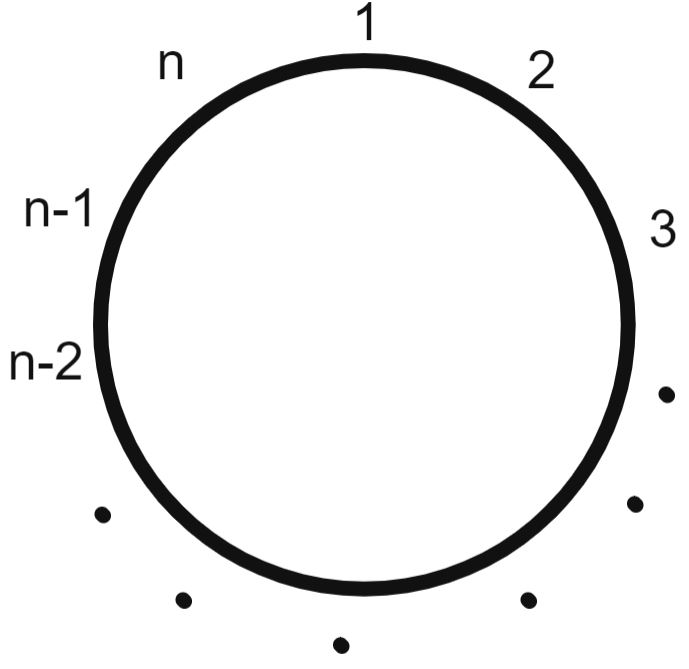
\includegraphics[width=\linewidth]{sol3} %тут поменять имя пикчи
    \end{figure}
    \end{minipage}
\end{minipage}

\textbf{Дефолтные математические знаки и символы:}\\
$\geqslant$,
$\leqslant$,
$a^{b}$,
$x_{i}$,
$\sqrt{a}$,
$\frac{a}{b}$,
$\displaystyle \frac{a}{b}$,
$\cdot$
$\;\Rightarrow\;$,
$\;\Leftrightarrow\;$,
$1{,}2$.
О промежутках:
$a\!b$,
$a\,b$,
$a\:b$,
$a\;b$,
$a\quad b$.

\textbf{Стандартные система и совокупность уравнений / неравенств:}\\
$\left\{
\begin{aligned}
f(x) &= 0 \\
g(x) &= 1
\end{aligned}\right.$

$\left[\begin{aligned}
&\left\{\begin{aligned}
f(x) &\geqslant a \\
g(x) &= b
\end{aligned}\right.\\
&\left\{\begin{aligned}
f(x) &< a \\
g(x) &= -b
\end{aligned}\right.
\end{aligned}\right.$

\subsection*{\textcolor{Emerald}{\textbf{Не математическое, но полезное:}}}
% комментарий в любом месте документа, который нигде не будет видно. Можно использовать для написания заметок-вопросов по задачам
\textbf{Пример таблицы:}

\begin{tabular}{|c|c|c|}
\hline
    $a$ & $b$ & текст
\\\hline
    $c$ & $d$ & мораль
\\\hline
\end{tabular}\\

\textbf{Отступы:} между\smallskip\\ строками\medskip\\ \textbf{Тире} --- это три дефиса.\\
\textbf{Списки:}
\begin{mylist}
\item [$\bullet$] это был пункт а
\item [2)] а это уже пункт номер 2 с изменённым заголовком
\end{mylist}

\subsection*{\textcolor{Emerald}{\textbf{Всё, неупомянутое выше (или если просто что-то не так):}}}
\begin{mylist}
\item [$\bullet$] Решение отдельных вопросов касательно ТеХа нужно искать в \href{https://www.mccme.ru/free-books/llang/newllang.pdf}{Львовском}.

\item [$\bullet$] Найти произвольный символ, который нужен, можно в \href{http://detexify.kirelabs.org/classify.html}{Detexify}.

\item [$\bullet$] Если возникли сомнения при решении, ответ практически ко всем задачам можно проверить с помощью \href{https://www.wolframalpha.com/}{WolframAlpha}.

\item [$\bullet$] Если в задаче нужно создать картинку, то лучше пока отложить эту задачу. Все графики планируется централизованно нарисовать (или перерисовать) в геогебре.

\item [\textcolor{brown}{\textbf{!!}}] Важно ставить \textcolor{red}{\textbf{$\spadesuit$}}
(или просто red) в тело задачи в случае серьёзных вопросов к решению и какой-то вопиющей лажи.

\item [\textcolor{brown}{\textbf{!!}}] Важно ставить \textcolor{olive}{\textbf{$\spadesuit$}}
(или просто olive) в тело задачи в случае не самого удачного текста и кривых отступов.
\end{mylist}

\subsection*{\textcolor{Violet}{\textbf{Комментарии:}}}% а также невидимые комментарии - так можно оставлять заметки-вопросы прямо в задаче, чтобы потом было понятно, в чём вопрос.
\begin{mylist}
\item [$\skull$] Переставлять задачи местами --- очень плохая идея.

\item [$\smiley$] При двойном клике по тексту pdf справа происходит автоматический переход к этому месту в латех-коде, а для обратного перехода можно нажать стрелку вправо (висит сверху между pdf и латех-кодом).

\item [$\smiley$] Если есть размышления, дописывать red/olive к задаче или не дописывать, то лучше всё-таки дописать.

\item [$\skull$] Самое плохое, что можно сделать --- написать в любое поле из трёх (НаписанноеРешение/ВерныйОтвет/Подсказка) только половину того, что надо, никак это не отметить, и потом пойти дальше.\\ Нужно в этот момент писать red/olive в случайном месте задачи, чтобы потом вычислить это с помощью Ctrl+F по всему документу (и это то, что потом будет делаться долго и тщательно)
\end{mylist}

\newpage
\setcounter{num}{1539}

\hypertarget{10.5}{{\centering\section*{\bigskip\\\textcolor{Blue}{\hyperlink{start2}{\textcolor{Blue}{10.5}} Производная.}\vspace{-5mm}}}}

\begin{problem}{Свойства последовательностей}{10.5.1}{10A}{(лёгкая)}
{Последовательность $(y_n)$ задана рекуррентно: $y_1 = 1$, $y_2 = 2$, $y_n = 6y_{n - 1} - 8y_{n - 2}$. Задать эту последовательность аналитически (то есть, написать, чему равно $y_n$)}
{НаписанноеРешение}
{ВерныйОтвет}{Подсказка}
\end{problem}

\begin{problem}{Свойства последовательностей}{10.5.1}{10A}{(лёгкая)}
{Последовательность $(y_n)$ задана рекуррентно: $y_1 = y_2 = c$, $y_n = y_{n - 2}^2 + 7y_{n - 1} - 7$. При каких значениях параметра $c$ данная последовательность будет постоянна? (равна одной и той же константе независимо от $n$)}
{НаписанноеРешение}
{ВерныйОтвет}{Подсказка}
\end{problem}

\begin{problem}{Свойства последовательностей}{10.5.1}{10A}{(лёгкая)}
{Исследовать на ограниченность (снизу и сверху) последовательность\\ \hspace*{6cm}$\displaystyle y_n = \frac{1}{1} + \frac{1}{2} + \frac{1}{3} + \ldots + \frac{1}{n}$.}
{НаписанноеРешение}
{ВерныйОтвет}{Подсказка}
\end{problem}

\begin{problem}{Свойства последовательностей}{10.5.1}{10A}{*}
{Исследовать на ограниченность (снизу и сверху) последовательность\\ \hspace*{5cm}$\displaystyle y_n = \frac{1}{\sqrt{1}} + \frac{1}{\sqrt{2}} + \frac{1}{\sqrt{3}} + \ldots + \frac{1}{\sqrt{n}}$.}
{НаписанноеРешение}
{ВерныйОтвет}{Подсказка}
\end{problem}

\begin{problem}{Свойства последовательностей}{10.5.1}{10A}{*}
{Исследовать на ограниченность (снизу и сверху) последовательность\\ \hspace*{5.5cm}$\displaystyle y_n = \frac{1}{1^2} + \frac{1}{2^2} + \frac{1}{3^2} + \ldots + \frac{1}{n^2}$.}
{НаписанноеРешение}
{ВерныйОтвет}{Подсказка}
\end{problem}

\begin{problem}{Свойства последовательностей}{10.5.1}{10A}{(лёгкая)}
{Исследовать на монотонность последовательность $\displaystyle \,y_n = \frac{n^2}{9^n}$.}
{НаписанноеРешение}
{ВерныйОтвет}{Подсказка}
\end{problem}

\begin{problem}{Свойства последовательностей}{10.5.1}{10A}{*}
{Исследовать на монотонность последовательность $\displaystyle \,y_n = \frac{n^2}{4{,}04^n}$.}
{НаписанноеРешение}
{ВерныйОтвет}{Подсказка}
\end{problem}

\begin{problem}{Предел числовой последовательности, сходимость и расходимость.}{10.5.2}{10A}{(лёгкая)}
{Найти предел (при $n \to \infty$) последовательности $\displaystyle \,g_n = \frac{3}{n - 5}$.}
{НаписанноеРешение}
{ВерныйОтвет}{Подсказка}
\end{problem}

\begin{problem}{Предел числовой последовательности, сходимость и расходимость.}{10.5.2}{10A}{(лёгкая)}
{Найти предел (при $n \to \infty$) последовательности $\displaystyle \,x_n = \frac{2}{n^2 + 4}$.}
{С ростом $n$ знаменатель дроби стремится к бесконечности, числитель равен 2. Значит, дробь стремится к 0 и предел последовательности равен нулю.}
{Предел последовательности $x_n = \frac{2}{n^2 + 4}$ равен нулю.}{К чему стремится знаменатель дроби с ростом $n$?}
\end{problem}

\begin{problem}{Предел числовой последовательности, сходимость и расходимость.}{10.5.2}{10A}{(лёгкая)}
{Найти предел (при $n \to \infty$) последовательности $\displaystyle \,y_n = \frac{2n}{n + 1}$.}
{Поскольку $n \neq 0$, разделим и числитель, и знаменатель дроби на $n$. Получаем $y_n = \frac{2}{1 + \frac1n}$. $\frac1n$ c ростом $n$ стремится к 0, поэтому $y_n$ стремится к $\frac21 = 2$.\\
\textbf{Альтернативное решение:} $y_n = \frac{2n + 2}{n + 1} - \frac{2}{n + 1} = 2 - \frac{2}{n + 1}$, эта дробь стремится к нулю, и предел последовательности также получается равным двум.}
{Предел последовательности $y_n = \frac{2n}{n + 1}$ равен 2.}{Перепиши дробь в другом виде или используй стандартный приём с делением числителя и знаменателя на $n^k$.}
\end{problem}

\begin{problem}{Предел числовой последовательности, сходимость и расходимость.}{10.5.2}{10A}{(лёгкая)}
{Найти предел (при $n \to \infty$) последовательности $\displaystyle s_n = \frac{3n}{10 - n}$.}
{Перепишем дробь так, чтобы $n$ осталось только в знаменателе: \\$\displaystyle s_n = \frac{3n}{10 - n} = \frac{30 - (30 - 3n)}{10 - n} = \frac{30}{10 - n} - \frac{30 - 3n}{10 - n} = \frac{30}{10 - n} - 3\;$ ($n \neq 10$)\\
Ищем предел: $\displaystyle \lim_{n \to \infty} s_n = \lim_{n \to \infty}\left(\frac{30}{10 - n} - 3\right) = \lim_{n \to \infty}\left(\frac{30}{10 - n}\right) - \lim_{n \to \infty}3 = 0 - 3 = -3$.\\
Итого, предел последовательности равен $-3$.}
{Предел последовательности $\displaystyle s_n = \frac{3n}{10 - n}$ равен $-3$.}{Нужно избавиться от $n$ в числителе, переписав дробь в другом виде.}
\end{problem}

\begin{problem}{Предел числовой последовательности, сходимость и расходимость.}{10.5.2}{10A}{(лёгкая)}
{Найти предел (при $n \to \infty$) последовательности $\displaystyle \,t_n = \frac{2n^2 + 7}{3n^2 + 10}$.}
{Поскольку $n \neq 0$, поделим и числитель, и знаменатель дроби на $n^2$.\smallskip\\ Тогда получим $\displaystyle t_n = \frac{2 + \frac{7}{n^2}}{3 + \frac{10}{n^2}}$. C ростом $n$ числитель стремится к 2, а знаменатель~--- к трём. То есть $t_n \to \frac23$, и пределом данной последовательности является $\frac23$.}
{Предел последовательности $t_n = \frac{2n^2 + 7}{3n^2 + 10}$ равен $\frac23$.}{Раздели числитель и знаменатель данной дроби на $n^k$.}
\end{problem}

\begin{problem}{Предел числовой последовательности, сходимость и расходимость.}{10.5.2}{10A}{(лёгкая)}
{Найти предел (при $n \to \infty$) последовательности $\displaystyle \,w_n = \frac{0{,}14n^2 - 2{,}5n + 36}{7n^2 + 8n + 9}$.}
{НаписанноеРешение}
{ВерныйОтвет}{Подсказка}
\end{problem}

\begin{problem}{Предел числовой последовательности, сходимость и расходимость.}{10.5.2}{10A}{(лёгкая)}
{Найти предел (при $n \to \infty$) последовательности $\displaystyle \,z_n = \frac{5n + 3}{n^2 - 5n + 4}$.}
{НаписанноеРешение}
{ВерныйОтвет}{Подсказка}
\end{problem}

\begin{problem}{Предел числовой последовательности, сходимость и расходимость.}{10.5.2}{10A}{(лёгкая)}
{Привести пример последовательности, которая ограничена сверху, ограничена снизу, но не сходится ни к одному пределу.}
{Примером такой последовательности может являться последовательность $0, 1, -1, 0, 1, -1, 0, 1, -1, 0, 1, -1 ,\ldots\;$ \\Действительно, данная последовательность ограничена и сверху и снизу (не превышает $1$ по модулю), но сходимость на бесконечности отсутствует.\\ Также её можно задать явно: $\displaystyle a_n = n - 1 - 3\left\lfloor\frac{n}{3}\right\rfloor$, где $\lfloor x\rfloor$~--- целая часть числа $x$ (floor function).\smallskip\\
Другим, более наглядным примером, может быть <<склеивание>> двух сходящихся последовательностей. Например: пусть $s_n = \frac{1}{2^n}$, $\,t_n = 2 - \frac{1}{3^n}$.\\ Очевидно, что $\forall n\; s_n > 0$ и $s_n \leqslant \frac12$, а также что $t_n \geqslant \frac53$ и $t_n < 2$.\\
Поэтому, если определить нашу последовательность как $\;\begin{cases}
a_{n} = s_{\frac {n+1}{2}}, \text{ если } n\!\!\not\vdots \,2\\
a_n = t_{\frac n2}, \text{ если } n \,\vdots\, 2
\end{cases}$\\ (то есть, нечётные члены нашей последовательности~--- последовательность $s_n$, а чётные~--- последовательность $t_n$), то мы получим последовательность, которая ограничена и сверху и снизу (2 и 0), а сходиться к одному пределу не может\\ (говорить, что она сходится сразу к двум пределам~--- 0 и 2 некорректно, так как по теореме Вейерштрасса предел может быть только один).}
{Механизм для построения подобных последовательностей~--- <<склейка>> нескольких последовательностей в одну. В этом случае ограниченность остаётся, а сходимости уже не будет.}{Подсказка}
\end{problem}

\begin{problem}{Предел функции в бесконечности и в точке.}{10.5.3}{10A}{(лёгкая)}
{Вычислить $\displaystyle \lim_{x \to \infty}\frac{12x^2 + 14x - 3}{5 - 3x - 2x^2}$.}
{Используем стандартный приём: поделим и числитель, и знаменатель дроби на $x^2$: так как $x\to\infty$, $x \neq 0$. Получаем:\\
$\displaystyle \lim_{x \to \infty}\frac{12x^2 + 14x - 3}{5 - 3x - 2x^2} = \displaystyle \lim_{x \to \infty}\frac{12 + \frac {14}{x} - \frac{3}{x^2}}{\frac{5}{x^2} - \frac 3x - 2}$.\\ Воспользуемся тем фактом, что отношение пределов есть предел отношения (если пределы существуют и предел знаменателя не равен 0). Следовательно,\\
$\displaystyle \lim_{x \to \infty}\frac{12 + \frac {14}{x} - \frac{3}{x^2}}{\frac{5}{x^2} - \frac 3x - 2} = \cfrac{\lim\limits_{x \to \infty} \left(12 + \frac {14}{x} - \frac{3}{x^2}\right)}{\lim\limits_{x \to \infty}\left( \frac{5}{x^2} - \frac 3x - 2\right)} = \frac{12 + 0 - 0}{0 - 0 - 2} = \frac{12}{-2} = -6$.}
{$\displaystyle \lim_{x \to \infty}\frac{12x^2 + 14x - 3}{5 - 3x - 2x^2} = -6$.}{Необходимо поделить и числитель, и знаменатель дроби на $x^2$.}
\end{problem}

\begin{problem}{Предел функции в бесконечности и в точке.}{10.5.3}{10A}{(лёгкая)}
{Вычислить $\displaystyle \lim_{x \to -1}\frac{8(x + 1) - 5(x + 1)^2 - 3}{(x + 1)^2 - 5(x + 1)^3 - 2(x + 1) + 10}$.}
{Присмотримся повнимательнее к данному выражению.\\ При $x \to -1$, $x + 1 \to 0$. Значит, и $(x + 1)^n \to 0$ ($n\in \mathbb{N}$). Но это означает, что числитель данной дроби стремится к $-3$, а знаменатель~--- к $10$.\\ Следовательно, пределом данного выражения является число $\frac{-3}{10} = -0{,}3$.}
{$\displaystyle \lim_{x \to -1}\frac{8(x + 1) - 5(x + 1)^2 - 3}{(x + 1)^2 - 5(x + 1)^3 - 2(x + 1) + 10} = -0{,}3$.}{К чему стремятся числитель и знаменатель дроби?}
\end{problem}

\begin{problem}{Предел функции в бесконечности и в точке.}{10.5.3}{10A}{(лёгкая)}
{Вычислить $\displaystyle \lim_{x \to 1} (x^3 + 3x^2 - 4x + 2)$.}
{НаписанноеРешение}
{ВерныйОтвет}{Подсказка}
\end{problem}

\begin{problem}{Предел функции в бесконечности и в точке.}{10.5.3}{10A}{(лёгкая)}
{Вычислить $\displaystyle \lim_{x \to 3}\frac{\cos (\pi(x + 1))}{\sqrt{x - 2}}$.}
{НаписанноеРешение}
{ВерныйОтвет}{Подсказка}
\end{problem}

\begin{problem}{Предел функции в бесконечности и в точке.}{10.5.3}{10A}{(лёгкая)}
{Вычислить $\displaystyle \lim_{x \to -2}\frac{x^2 - 4}{3x + 6}$.}
{$\displaystyle \lim_{x \to -2}\frac{x^2 - 4}{3x + 6} = \lim_{x \to -2}\frac{(x - 2)(x + 2)}{3(x + 2)}$. При $x \to -2$, $x + 2 \to 0$, однако $x + 2 \neq 0$, поэтому мы можем сократить дробь на $x + 2$.\smallskip\\ Следовательно,
$\displaystyle \lim_{x \to -2}\frac{(x - 2)(x + 2)}{3(x + 2)} = \lim_{x \to -2}\frac{x - 2}{3} = \frac{-2 -2}{3} = -\frac43$.}
{$\displaystyle \lim_{x \to -2}\frac{x^2 - 4}{3x + 6} = -\frac43$.}{Разложи на множители числитель и знаменатель.}
\end{problem}

\begin{problem}{Предел функции в бесконечности и в точке.}{10.5.3}{10A}{*}
{Вычислить $\displaystyle \lim_{x \to 7}\frac{\sqrt{x + 2} - 3}{x - 7}$.}
{Заметим, что и предел знаменателя, и предел числителя равны 0. Поэтому воспользоваться отношением пределов не получится.\\ Используем хитрость: домножим и числитель, и знаменатель дроби на $\sqrt{x + 2} + 3$ (при $x \to 7$ стремится к 6, не равно 0). Тогда:\\
$\displaystyle \lim_{x \to 7}\frac{\sqrt{x + 2} - 3}{x - 7} = \lim_{x \to 7}\frac{(\sqrt{x + 2} - 3)\cdot(\sqrt{x + 2} + 3)}{(x - 7)\cdot(\sqrt{x + 2} + 3)} = \lim_{x \to 7}\frac{x + 2 - 9}{(x - 7)\cdot(\sqrt{x + 2} + 3)}$.\smallskip\\
Поскольку $x\!\to\!7$, $x \!-\! 7 \!\to\! 0$. Но $x\! -\! 7 \neq 0$, а следовательно, на $x\! -\! 7$ можно поделить.\\
$\Rightarrow\, \displaystyle \lim_{x \to 7}\frac{x + 2 - 9}{(x \!-\! 7)\cdot(\sqrt{x \!+\! 2} + 3)} = \lim_{x \to 7}\frac{1}{\sqrt{x \!+\!2} + 3} = \frac{\lim\limits_{x \to 7}\,1}{\lim\limits_{x \to 7}\sqrt{x \!+\! 2} + 3} = \frac{1}{\sqrt{7 \!+\! 2} + 3} = \frac16$.}
{$\displaystyle \lim_{x \to 7}\frac{\sqrt{x + 2} - 3}{x - 7} = \frac16$.

}{Надо домножить на сопряжённое (хотя в знаменателе и нет корня).}
\end{problem}

\begin{problem}{Предел функции в бесконечности и в точке.}{10.5.3}{10A}{(лёгкая)}
{Вычислить $\displaystyle \lim_{x \to 3}\frac{\sqrt{4x - 3} - 3}{x - 3}$.}
{НаписанноеРешение}
{ВерныйОтвет}{Подсказка}
\end{problem}

\begin{problem}{Предел функции в бесконечности и в точке.}{10.5.3}{10A}{(лёгкая)}
{Вычислить $\displaystyle \lim_{x \to 5{,}5}\frac{\sqrt{2x + 5} - 4}{4x - 22}$.}
{НаписанноеРешение}
{ВерныйОтвет}{Подсказка}
\end{problem}

\begin{problem}{Предел функции в бесконечности и в точке.}{10.5.3}{10A}{(лёгкая)}
{Вычислить $\displaystyle \lim_{x \to \frac{4}{3}}\frac{\sqrt{\frac{4x}{3} + 20} - \frac{14}{3}}{6x - 8}$.}
{При $x \to \frac43$ подкоренное выражение стремится к $\frac{196}{9}$, а значит, числитель стремится к 0. Знаменатель, в свою очередь, также стремится к нулю: возникает неопределённость вида $\frac00$. Домножим на сопряжённое~--- $\sqrt{\frac{4x}{3} + 20} + \frac{14}{3}$ и числитель, и знаменатель (при $x \to \frac43$ стремится к $\frac{28}{3}$):\\
Получаем $\displaystyle \lim_{x \to \frac{4}{3}}\frac{\sqrt{\frac{4x}{3} + 20} - \frac{14}{3}}{6x - 8} = \lim_{x \to \frac{4}{3}}\frac{\left(\sqrt{\frac{4x}{3} + 20} - \frac{14}{3}\right)\!\left(\sqrt{\frac{4x}{3} + 20} + \frac{14}{3}\right)}{(6x - 8)\left(\sqrt{\frac{4x}{3} + 20} + \frac{14}{3}\right)} =$ \\
$=\displaystyle\lim_{x \to \frac{4}{3}}\frac{\frac{4x}{3} + 20 - \frac{196}{9}}{2\,(3x - 4)\!\left(\sqrt{\frac{4x}{3} + 20} + \frac{14}{3}\right)} = \lim_{x \to \frac{4}{3}}\frac{\frac{4}{9}(3x - 4)}{2\,(3x - 4)\!\left(\sqrt{\frac{4x}{3} + 20} + \frac{14}{3}\right)} = $\\
$=\displaystyle \lim_{x \to \frac{4}{3}}\frac{\frac{4}{9}}{2\!\left(\sqrt{\frac{4x}{3} + 20} + \frac{14}{3}\right)} = \frac{\frac49}{2\cdot\frac{28}{3}} = \frac{4}{6\cdot28} = \frac{1}{42}$.}
{$\,\displaystyle \lim_{x \to \frac{4}{3}}\frac{\sqrt{\frac{4x}{3} + 20} - \frac{14}{3}}{6x - 8} = \frac{1}{42}$.}{Для раскрытия неопределённости вида $\frac00$ нужно домножить на сопряжённое.}
\end{problem}

\begin{problem}{Предел функции в бесконечности и в точке.}{10.5.3}{10A}{(лёгкая)}
{Вычислить $\displaystyle \lim_{x \to \infty}\frac{\sin x}{x}$.}
{НаписанноеРешение}
{ВерныйОтвет}{Подсказка}
\end{problem}

\begin{problem}{Предел функции в бесконечности и в точке.}{10.5.3}{10A}{*}
{Вычислить $\displaystyle \lim_{x \to 0}\frac{\sin x}{x}$.}
{НаписанноеРешение}
{ВерныйОтвет}{Подсказка}
\end{problem}

\begin{problem}{Определение производной, связь с непрерывностью.}{10.5.6}{10A}{(лёгкая)}
{Пользуясь определением производной, $\displaystyle f'(x) = \lim_{\Delta x \to 0}\frac{f(x + \Delta x) - f(x)}{\Delta x}$,\\ найти производную функции $f(x) = C$ (функция равна константе).}
{НаписанноеРешение}
{ВерныйОтвет}{Подсказка}
\end{problem}

\begin{problem}{Определение производной, связь с непрерывностью.}{10.5.6}{10A}{(лёгкая)}
{Пользуясь определением производной, $\displaystyle f'(x) = \lim_{\Delta x \to 0}\frac{f(x + \Delta x) - f(x)}{\Delta x}$,\\ найти производную функции $f(x) = x^n$.}
{НаписанноеРешение}
{ВерныйОтвет}{Подсказка}
\end{problem}

\begin{problem}{Определение производной, связь с непрерывностью.}{10.5.6}{10A}{(лёгкая)}
{Пользуясь определением производной, $\displaystyle f'(x) = \lim_{\Delta x \to 0}\frac{f(x + \Delta x) - f(x)}{\Delta x}$,\\ найти производную функции $\displaystyle f(x) = \frac{1}{x}$.}
{Найдём производную по определению: $\displaystyle f'(x) = \lim_{\Delta x \to 0}\frac{\frac{1}{x + \Delta x} - \frac{1}{x}}{\Delta x} =$\vspace{-2mm}\\ $\displaystyle\lim_{\Delta x \to 0}\frac{\frac{x - (x + \Delta x)}{x(x + \Delta x)}}{\Delta x} = \lim_{\Delta x \to 0}\frac{\frac{-\Delta x}{x(x + \Delta x)}}{\Delta x}$.\medskip\\ Поскольку $\Delta x \neq 0$, можем на него поделить и числитель, и знаменатель:\\
$\displaystyle \lim_{\Delta x \to 0}\frac{\frac{-\Delta x)}{x(x + \Delta x)}}{\Delta x} = \lim_{\Delta x \to 0}\frac{\frac{-1}{x(x + \Delta x)}}{1} = \lim_{\Delta x \to 0} -\frac{1}{x(x + \Delta x)} = \lim_{\Delta x \to 0} -\frac{1}{x^2 + x\Delta x} = -\frac{1}{x^2}$.}
{Для функции $f(x) = \displaystyle \frac1x$ производная равна $\displaystyle \left(\frac{1}{x}\right)' = -\frac{1}{x^2}$.}{Подставить $\displaystyle f(x) = \frac1x$ и не бояться трёхэтажных дробей.}
\end{problem}

\begin{problem}{Определение производной, связь с непрерывностью.}{10.5.6}{10A}{(лёгкая)}
{Пользуясь определением производной, $\displaystyle f'(x) = \lim_{\Delta x \to 0}\frac{f(x + \Delta x) - f(x)}{\Delta x}$,\\ найти производную функции $\displaystyle f(x) = \frac{1}{x^2}$.}
{НаписанноеРешение}
{ВерныйОтвет}{Подсказка}
\end{problem}

\begin{problem}{Определение производной, связь с непрерывностью.}{10.5.6}{10A}{*}
{Пользуясь определением производной, $\displaystyle f'(x) = \lim_{\Delta x \to 0}\frac{f(x + \Delta x) - f(x)}{\Delta x}$,\\ найти производную функции $f(x) = \sqrt{x}$.}
{НаписанноеРешение}
{ВерныйОтвет}{Подсказка}
\end{problem}

\begin{problem}{Определение производной, связь с непрерывностью.}{10.5.6}{10A}{*}
{Привести два примера функций, являющихся непрерывными, но не дифференцируемыми (в какой-то точке).}
{Функция непрерывна, если она меняется плавно, без скачков.\\ Производная же показывает скорость изменения функции.\\ То есть нам нужно придумать ситуацию, в которой функция меняет значения плавно, но её скорость изменения не определена.\smallskip\\ Первый пример непрерывной, но не дифференцируемой (в нуле) функции: $y = |x|$.
Действительно, хоть в нуле и минимум функции, нельзя сказать, что $y'(0) = 0$, поскольку везде левее функция ведёт себя как $y = -x$, и её производная равна $-1$, а везде правее функция ведёт себя как $y = x$, и её производная равна $1$. Производная, являясь пределом, в данном случае зависит от того, с какой стороны мы приближаемся к нулю. А значит, её значение не определено.\smallskip\\
Второй пример: нужна функция, в область определения производной которой не входит 0. Оказывается, что примером такой функции является $y = \sqrt[3]{x}$.\\ В самом деле, согласно общей формуле, $y'(x) = \frac{1}{3\sqrt[3]{x^2}}$. В точке $x = 0$ производная не определена. Из графика понятно, что происходит: в этой точке касательная к графику функции $y = \sqrt[3]{x}$ является вертикальной прямой, а для того, чтобы функция была дифференцируема, мы должны иметь $f(x) \sim f'(x_0)(x - x_0) + f(x_0)$.\\
Конечно, можно придумать и много других примеров, но везде будет реализован один из этих сценариев: либо скорость изменения на двух концах разная (легко получить склеиванием двух функций), либо скорость изменения <<равна $\pm\infty$>>.}
{Два подходящих примера~--- функции $y = |x|$ и $y = \sqrt[3]{x}$: данные функции непрерывны, но значение производной в нуле у них не определено.}{Один из случаев получается, когда скорость изменения у функции слева и справа от точки разная.}
\end{problem}

\begin{problem}{Определение производной, связь с непрерывностью.}{10.5.6}{10A}{*}
{Привести пример функции, производная которой не определена для всех целых $x$, а для всех остальных вещественных чисел равна 1.}
{Исходя из того, что производная не определена для всех целых чисел, можно понять, что данная функция нам пока не встречалась (не прямая, не многочлен, не корень, не гипербола).\smallskip\\ Попробуем восстановить график этой функции, зная, как выглядит производная.\\ Поскольку производная равна 1, сама функция для нецелых $x$ должна вести себя как $y = x$. Причём, так как на всём интервале $(0; 1)$ производная равна 1, на этом интервале функция обязательно равна $y = x + c_0$. На любом другом интервале с целыми концами $(n; n\!+\!1)$ по тем же соображениям $y = x + c_n$. Константы здесь нам пока неизвестны (понятно лишь, что в каждой целой точке нужно разрывать линию, чтобы производная была не определена). Любая функция такого вида подойдёт под условие (то есть нужно лишь чтобы $c_n \neq c_{n-1}$ для всех целых $n$).\smallskip\\ В качестве примера можно взять $c_n = -n$ для всех целых $n$, и получаемая в этом случае функция $f$ имеет название: это функция дробной части числа.\\ Она определяется как $f(a + x) = x$, где $a \in \mathbb{Z}$~--- любое целое число, а $x \in [0; 1)$.\\
То есть: $f(1{,}23) = 0{,}23$, $\,f(4\frac59) = \frac59$, $\,f(2) = 0$, $\,f(-0{,}77) = 0{,}23$.\\ Её график выглядит как зубья пилы, а производная удовлетворяет требованиям.}
{Данная функция~--- функция целой части числа или другая функция такого типа, график которой выглядит как <<зубья пилы>>.}{Если на каком-то интервале для функции известна производная, то её вид на этом интервале известен \textit{с точностью до константы.}}
\end{problem}

\begin{problem}{Определение производной, связь с непрерывностью.}{10.5.6}{10A}{*}
{Привести пример функции, которая определена для всех $x$, но не является непрерывной ни в одной точке $x_0 \in \mathbb{R}$.}
{НаписанноеРешение}
{ВерныйОтвет}{Подсказка}
\end{problem}

\begin{problem}{Формулы и правила дифференцирования.}{10.5.7}{10A}{*}
{Пользуясь определением производной, $\displaystyle f'(x) = \lim_{\Delta x \to 0}\frac{f(x + \Delta x) - f(x)}{\Delta x}$,\\ определением замечательного предела, и формулой синуса суммы, найти\\ производную функции $f(x) = \sin x$.}
{НаписанноеРешение}
{ВерныйОтвет}{Подсказка}
\end{problem}

\begin{problem}{Формулы и правила дифференцирования.}{10.5.7}{10A}{*}
{Пользуясь определением производной, $\displaystyle f'(x) = \lim_{\Delta x \to 0}\frac{f(x + \Delta x) - f(x)}{\Delta x}$,\\ определением замечательного предела, формулой косинуса суммы, и в частности, формулой косинуса двойного угла, найти производную функции $f(x) = \cos x$.}
{Для нахождения производной, распишем её по определению: \\$\displaystyle (\cos x)' = \lim_{\Delta x \to 0}\frac{\cos(x + \Delta x) - \cos(x)}{\Delta x}$. Используем формулу косинуса суммы:\\ $\displaystyle (\cos x)' = \lim_{\Delta x \to 0}\frac{\cos x \cos\Delta x - \sin x \sin\Delta x - \cos(x)}{\Delta x} = \cos x \cdot \lim_{\Delta x \to 0}\frac{\cos\Delta x - 1}{\Delta x} -$ \\ $-\displaystyle \sin x \cdot \lim_{\Delta x \to 0}\frac{\sin\Delta x}{\Delta x}$. По свойствам первого замечательного предела, второй предел равен 1. Поэтому $\displaystyle (\cos x)' = \cos x \cdot \lim_{\Delta x \to 0}\frac{\cos\Delta x - 1}{\Delta x} - \sin x$. Согласно формуле для косинуса двойного угла, $\cos 2x = 1 - 2\sin^2 x$, откуда $\cos\Delta x - 1 = -2\sin^2\frac{\Delta x}{2} \;\Rightarrow$ \\ $\displaystyle \cos'(x) = \cos x\, \cdot\! \lim_{\Delta x \to 0}\!\!\frac{-2\sin^2\frac{\Delta x}{2}}{\Delta x} - \sin x = -\!\sin x + \cos x \,\cdot\! \lim_{\Delta x \to 0}\!\!\frac{\sin\frac{\Delta x}{2}}{\frac{\Delta x}{2}} \cdot\! \lim_{\Delta x \to 0} \!\!\left(-\!\sin\tfrac{\Delta x}{2}\right) = $ \\ $-\sin x + \cos x \cdot 1 \cdot 0 = -\sin x$. Итого, $(\cos x)' = -\sin x$.}
{$(\cos x)' = -\sin x$.}{Формулу косинуса двойного угла стоит использовать после всех преобразований, чтобы заменить оставшееся выражение $\cos \phi - 1$ на более удачное.}
\end{problem}

\begin{problem}{Формулы и правила дифференцирования.}{10.5.7}{10A}{*}
{Пользуясь определением производной, $\displaystyle f'(x) = \lim_{\Delta x \to 0}\frac{f(x + \Delta x) - f(x)}{\Delta x}$,\\ определением замечательного предела, и формулой тангенса суммы, найти\\ производную функции $f(x) = \tg x$.}
{НаписанноеРешение}
{ВерныйОтвет}{Подсказка}
\end{problem}

\begin{problem}{Формулы и правила дифференцирования.}{10.5.7}{10A}{*}
{Пользуясь определением производной, $\displaystyle f'(x) = \lim_{\Delta x \to 0}\frac{f(x + \Delta x) - f(x)}{\Delta x}$,\\ определением замечательного предела, и формулой котангенса суммы, найти\\ производную функции $f(x) = \ctg x$.}
{Для нахождения производной, распишем её по определению: \\$\displaystyle (\ctg x)' = \lim_{\Delta x \to 0}\frac{\ctg(x + \Delta x) - \ctg(x)}{\Delta x} = \lim_{\Delta x \to 0}\frac{\frac{\cos(x + \Delta x)}{\sin(x + \Delta x)} - \frac{\cos x}{\sin x}}{\Delta x}$.\smallskip\\ Теперь используем формулу синуса и косинуса суммы:\\ $\displaystyle (\ctg x)' = \lim_{\Delta x \to 0}\frac{\frac{\cos x \cos\Delta x - \sin x \sin\Delta x}{\sin x \cos\Delta x + \cos x \sin\Delta x} - \frac{\cos x}{\sin x}}{\Delta x} = \lim_{\Delta x \to 0}\tfrac{- \sin^2 x \sin\Delta x - \cos^2 x \sin\Delta x}{(\sin x \cos\Delta x + \cos x \sin\Delta x) \cdot \sin x \cdot \Delta x} =$\\ $\displaystyle \lim_{\Delta x \to 0}\tfrac{- (\sin^2 x + \cos^2 x) \cdot \sin\Delta x}{(\sin^2 x \cos\Delta x + \sin x\cos x \sin\Delta x) \cdot \Delta x} = \lim_{\Delta x \to 0}\tfrac{- 1}{\sin^2 x \cos\Delta x + \sin x\cos x \sin\Delta x} \cdot \lim_{\Delta x \to 0}\tfrac{\sin\Delta x}{\Delta x}$.\smallskip\\ По свойствам первого замечательного предела, второй предел равен 1.\\ Поэтому $\displaystyle (\ctg x)' = \lim_{\Delta x \to 0}\frac{- 1}{\sin^2 x \cos\Delta x + \sin x\cos x \sin\Delta x} = -\frac{1}{\sin^2 x \cdot 1} = -\frac{1}{\sin^2 x}$.}
{$\displaystyle (\ctg x)' = -\frac{1}{\sin^2 x}$.}{Следует написать определение производной, воспользоваться формулами синуса суммы и косинуса суммы, и привести всё к единому знаменателю.}
\end{problem}

\begin{problem}{Формулы и правила дифференцирования.}{10.5.7}{10A}{(лёгкая)}
{(Производная суммы равна сумме производных)\\ Пользуясь определением производной, $\displaystyle f'(x) = \lim_{\Delta x \to 0}\frac{f(x + \Delta x) - f(x)}{\Delta x}$, показать, что для любых дифференцируемых функций $f(x)$ и $g(x)$ выполнено равенство\medskip\\ \hspace*{6cm}$\displaystyle (f(x) + g(x))' = f'(x) + g'(x).$
%\smallskip\\\textbf{Комментарий:} дифференцируемой называется функция, производная которой определена (то есть для неё нет никаких проблем при вычислении предела).
}
{Используем определение производной: производная суммы функций равна $\displaystyle (f(x) + g(x))' = \lim_{\Delta x \to 0}\frac{f(x + \Delta x) + g(x + \Delta x) - (f(x) + g(x))}{\Delta x} =$ \smallskip\\ $\displaystyle \lim_{\Delta x \to 0}\frac{f(x + \Delta x) - f(x) + g(x + \Delta x) - g(x)}{\Delta x} = \lim_{\Delta x \to 0}\frac{f(x + \Delta x) - f(x)}{\Delta x} \,+ $\smallskip\\ $\displaystyle+ \lim_{\Delta x \to 0}\frac{g(x + \Delta x) - g(x)}{\Delta x} = f'(x) + g'(x)$~--- сумма производных. Доказано.}
{Смотри выкладки выше.}{Написать производную функции $f(x) + g(x)$ по определению.}
\end{problem}

\begin{problem}{Формулы и правила дифференцирования.}{10.5.7}{10A}{(лёгкая)}
{(Константу можно вынести за знак производной)\\ Пользуясь определением производной, $\displaystyle f'(x) = \lim_{\Delta x \to 0}\frac{f(x + \Delta x) - f(x)}{\Delta x}$, показать, что для любой дифференцируемой функции $f(x)$ выполнено равенство \medskip\\ \hspace*{7.5cm}$\displaystyle (kf(x))' = kf'(x).$
%\smallskip\\\textbf{Комментарий:} дифференцируемой называется функция, производная которой определена (то есть для неё нет никаких проблем при вычислении предела).
}
{Используем определение производной для функции $kf(x)$: \\$(kf(x))' = \displaystyle \lim_{\Delta x \to 0}\frac{kf(x + \Delta x) - kf(x)}{\Delta x} = \lim_{\Delta x \to 0}\left(k\cdot\frac{f(x + \Delta x) - f(x)}{\Delta x}\right) = $\\$ \displaystyle = k\cdot\lim_{\Delta x \to 0}\frac{f(x + \Delta x) - f(x)}{\Delta x} = kf'(x)$. Доказано.}
{Смотри выкладки выше.}{Написать производную функции $kf(x)$ по определению.}
\end{problem}

\begin{problem}{Формулы и правила дифференцирования.}{10.5.7}{10A}{*}
{(Производная произведения)\\ Пользуясь определением производной, $\displaystyle f'(x) = \lim_{\Delta x \to 0}\frac{f(x + \Delta x) - f(x)}{\Delta x}$, показать, что для любых дифференцируемых функций $f(x)$ и $g(x)$ выполнено \medskip\\ \hspace*{5cm}$\displaystyle (f(x) \cdot g(x))' = f'(x) \cdot g(x) + f(x) \cdot g'(x).$
%\smallskip\\\textbf{Комментарий:} дифференцируемой называется функция, производная которой определена (то есть для неё нет никаких проблем при вычислении предела).
}
{Используем определение производной и тот факт, что $f(x + \Delta x) =  f(x) + \Delta f$:\\
$\displaystyle (f(x) \cdot g(x))' = \lim_{\Delta x \to 0}\frac{f(x + \Delta x) \cdot g(x + \Delta x) - f(x) \cdot g(x)}{\Delta x} =$\smallskip\\ $\displaystyle\lim_{\Delta x \to 0}\frac{(f(x) + \Delta f) \cdot (g(x) + \Delta g) - f(x) \cdot g(x)}{\Delta x} = \lim_{\Delta x \to 0}\frac{\Delta f \cdot g(x) + f(x) \cdot \Delta g + \Delta f\Delta g}{\Delta x}$\smallskip\\ $\displaystyle= \lim_{\Delta x \to 0}\frac{\Delta f \cdot g(x)}{\Delta x} + \lim_{\Delta x \to 0}\frac{f(x) \cdot \Delta g}{\Delta x} + \lim_{\Delta x \to 0}\frac{\Delta f\Delta g}{\Delta x} = g(x) \cdot \lim_{\Delta x \to 0}\frac{\Delta f}{\Delta x} + f(x) \cdot \lim_{\Delta x \to 0}\frac{\Delta g}{\Delta x} +$ \smallskip\\ $\displaystyle+ \lim_{\Delta x \to 0}\frac{\Delta f}{\Delta x} \cdot \frac{\Delta g}{\Delta x} \cdot \Delta x = g(x) \cdot f'(x) + f(x) \cdot g'(x) + f'(x)\cdot g'(x) \cdot \lim_{\Delta x \to 0} \Delta x =$ \smallskip\\
$f'(x) \cdot g(x) + f(x) \cdot g'(x)$.}
{Формула дифференцирования произведения имеет вид $(fg)' = f'g + fg'$.

}{Cтоит заметить, что $f(x + \Delta x) =  f(x) + \Delta f$.}
\end{problem}

\begin{problem}{Формулы и правила дифференцирования.}{10.5.7}{10A}{*}
{(Производная дроби)\\ Пользуясь определением производной, $\displaystyle f'(x) = \lim_{\Delta x \to 0}\frac{f(x + \Delta x) - f(x)}{\Delta x}$, показать, что для любой дифференцируемой $f(x)$ и дифференцируемой $g(x) \neq 0$ выполнено\\ \hspace*{5cm}$\displaystyle \left(\frac{f(x)}{g(x)}\right)' = \frac{f'(x) \cdot g(x) - f(x) \cdot g'(x)}{g^2(x)}.$
%\smallskip\\\textbf{Комментарий:} дифференцируемой называется функция, производная которой определена (то есть для неё нет никаких проблем при вычислении предела).
}
{НаписанноеРешение}
{ВерныйОтвет}{Стоит заметить, что $f(x + \Delta x) =  f(x) + \Delta f$.}
\end{problem}

\begin{problem}{Формулы и правила дифференцирования.}{10.5.7}{10A}{*}
{(Цепное правило)\\ Пользуясь определением производной, $\displaystyle f'(x) = \lim_{\Delta x \to 0}\frac{f(x + \Delta x) - f(x)}{\Delta x}$, показать, что для любых дифференцируемых функций $f(y)$ и $y(x)$ выполнено равенство\medskip\\ \hspace*{5cm}$\displaystyle (f(g(x)))' = f'(g(x)) \cdot g'(x).$
%\smallskip\\\textbf{Комментарий:} дифференцируемой называется функция, производная которой определена (то есть для неё нет никаких проблем при вычислении предела).
}
{НаписанноеРешение}
{ВерныйОтвет}{Подсказка}
\end{problem}

\begin{problem}{Формулы и правила дифференцирования.}{10.5.7}{10A}{(лёгкая)}
{Вычислить производную $f'(x)$ функции $f(x) = x^3 - x^2$.}
{Согласно таблице производных, $(x^n)' = nx^{n - 1}$.\\ В силу линейности производной, $f'(x) = (x^3 - x^2)' = (x^3)' - (x^2)' = 3x^2 - 2x$.}
{$f'(x) = 3x^2 - 2x$.}{Используй табличную производную $x^n$ и линейность производной.}
\end{problem}

\begin{problem}{Формулы и правила дифференцирования.}{10.5.7}{10A}{(лёгкая)}
{Вычислить производную $f'(x)$ функции $f(x) = \frac1x = x^{-1}$.}
{Согласно таблице производных, $(x^k)' = kx^{k - 1}$.\\ Поэтому $f'(x) = (\frac1x)' = (x^{-1})' = -x^{-2} = -\frac{1}{x^2}$.}
{$f'(x) = -\frac{1}{x^2}$.}{Используй табличную производную $x^k$.}
\end{problem}

\begin{problem}{Формулы и правила дифференцирования.}{10.5.7}{10A}{(лёгкая)}
{Вычислить производную $f'(x)$ функции $f(x) = 3\sqrt{x} = 3x^{\frac12}$.}
{Согласно таблице производных, $(x^k)' = kx^{k - 1}$. Используем тот факт, что константу можно вынести за знак производной, получаем, что $f'(x) = (3\sqrt{x})' =$ \\ $= (3\cdot x^{\frac12})' = 3\cdot (x^{\frac12})' = 3\cdot\frac12 \cdot x^{-\frac12} = \frac{3}{2\sqrt{x}}$.}
{$f'(x) = \frac{3}{2\sqrt{x}}$.}{Используй производную $x^k$ и вынеси константу за знак производной.}
\end{problem}

\begin{problem}{Формулы и правила дифференцирования.}{10.5.7}{10A}{(лёгкая)}
{Вычислить производную $f'(x)$ функции $f(x) = 2\sin x - 3\cos x$.}
{Согласно таблице производных, $(\sin x)' = \cos x$, а $(\cos x)' = -\sin x$. Используем линейность производной и получаем, что $f'(x) = (2\sin x - 3\cos x)' = 2\cdot(\sin x)' - 3\cdot(\cos x)' = 2\cdot\cos x - 3\cdot(-\sin x) = 2\cos x + 3\sin x$.}
{$f'(x) = 2\cos x + 3\sin x$.}{Используй табличные производные тригонометрических функций и линейность производной.}
\end{problem}

\begin{problem}{Производная n-ого порядка.}{10.5.8}{10A}{(лёгкая)}
{Найти $h''(-1)$, если $h(x) = 2x^5$.}
{Для начала находим первую производную функции $h(x)$:\\ $h'(x) = (2x^5)' = 2\cdot(x^5)' = 2\cdot5x^4 = 10x^4$. Теперь находим уже вторую производную, взяв производную ещё раз: $h''(x) = (h'(x))' = (10x^4)' = 10\cdot(x^4)' = 40x^3$.\\
Поскольку единственное, что нужно~--- найти значение этой функции $h''(x)$ в точке $x = -1$, подставляем: $h''(-1) = 40 \cdot (-1)^3 = -40$.}
{Вторая производная $h(x)$ в $-1$ равна $h''(-1) = -40$.}{Найти сначала первую, а потом вторую производную $h(x)$.}
\end{problem}

\begin{problem}{Производная n-ого порядка.}{10.5.8}{10A}{(лёгкая)}
{Найти $f''(x)$, если $f(x) = 3x^2 - \sin x$.}
{Для начала находим первую производную функции $f(x) = 3x^2 - \sin x$:\\ $f'(x) = (3x^2 - \sin x)' = 3\cdot(x^2)' - (\sin x)' = 3\cdot2x - \cos x = 6x - \cos x$.\\ Теперь находим уже вторую производную, взяв производную ещё раз:\\ $f''(x) = (f'(x))' = (6x - \cos x)' = 6 - (\cos x)' = 6 - (-\sin x) = 6 + \sin x$.}
{$f''(x) = 6 + \sin x$.}{Сначала найти первую, а уже потом вторую производную $f(x)$.}
\end{problem}

\begin{problem}{Производная n-ого порядка.}{10.5.8}{10A}{(лёгкая)}
{Найти $f'''(2)$, если $f(x) = 2x^4 - 5x^3 + 77x^2 - x + 2$.}
{Нам нужно найти третью производную в 2 от степенной функции $f$. Будем искать производные по порядку, начиная с первой:\\
$f'(x) = (2x^4 - 5x^3 + 77x^2 - x + 2)' = 2(x^4)' - 5(x^3)' + 77(x^2)' - x' = 8x^3 - 15x^2 + 154x - 1$.\\
$f''(x) = (8x^3 - 15x^2 + 154x - 1)' = 8(x^3)' - 15(x^2)' + 154x' = 24x^2 - 30x + 154$.\\
$f'''(x) = (24x^2 - 30x + 154)' = 24(x^2)' - 30x' = 48x - 30$.\smallskip\\
Итого, $f'''(x) = 48x - 30$. Поэтому $f'''(2) = 48\cdot2 - 30 = 66$.}
{Третья производная функции $f$ в точке 2 равна 66.}{Все три производные нужно найти по очереди.}
\end{problem}

\begin{problem}{Производная n-ого порядка.}{10.5.8}{10A}{(лёгкая)}
{Тело движется прямолинейно по закону $s(t) = 3t + 4$ ($s$~--- расстояние в метрах, $t$~--- время в секундах). Чему равна равнодействующая сила, действующая на тело?

}
{Найдём ускорение, с которым движется это тело.\\ Ускорение~--- вторая производная от расстояния, поэтому: $s'(t) = 3 \; \Rightarrow\; s''(t) = 0$.\\ Поэтому ускорение тела равно 0. Следовательно, по второму закону Ньютона, $F_{\text{равн}} = ma = m\cdot0 = 0$. Равнодействующая сила равна 0.}
{Действующая на тело равнодействующая сила равна нулю.}{Найти ускорение, с которым движется это тело.}
\end{problem}

\begin{problem}{Производная n-ого порядка.}{10.5.8}{10A}{(лёгкая)}
{На тело некоторой массы $m$ действует сила $F$, в результате чего оно движется по прямой, а его закон движения имеет вид $s(t) = -5t^2 + t + 3$ ($s$~--- расстояние в метрах, $t$~--- время в секундах).\\ Доказать, что сила $F$ постоянна и не меняется со временем.}
{НаписанноеРешение}
{ВерныйОтвет}{Подсказка}
\end{problem}

\begin{problem}{Производная n-ого порядка.}{10.5.8}{10A}{(лёгкая)}
{В некоторый момент времени пассажир автобуса двигался по прямой так, что его координата зависела от времени следующим образом: $x(t) = 1536 + 16t - t^2$ ($x$~--- расстояние в метрах, $t$~--- время в секундах). Ускоряется автобус или тормозит? Найти его ускорение. В какой момент времени автобус будет неподвижен?}
{Вычислим ускорение: найдем $a(t)$.\\ $a(t) = x''(t) = (1536 + 16t - t^2)'' = (16 - 2t)' = -2$. Таким образом, $a = -2$ м/с$^2$.\\ Поскольку ускорение отрицательно, автобус тормозит.\\ В тот момент времени, когда автобус будет неподвижен, его скорость будет равна нулю. Скорость мы уже нашли: $v(t) = x'(t) = 16 - 2t$. Отсюда получаем $t = 8$.\\ То есть автобус будет неподвижен через 8 с.}
{Автобус тормозит с постоянным ускорением $a = -2$ м/с$^2$, и в результате этого остановится через 8 секунд.}{Вычислить две производные.}
\end{problem}

\begin{problem}{Дифференцирование сложной функции.}{10.5.9}{10A}{(лёгкая)}
{Записать композицию $f(g(x))$ функций $f(x) = \sqrt[3]{x}$ и $g(x) = x^2 - 1$, и найти значение этой функции при $x = -3$.}
{НаписанноеРешение}
{ВерныйОтвет}{Подсказка}
\end{problem}

\begin{problem}{Дифференцирование сложной функции.}{10.5.9}{10A}{(лёгкая)}
{Записать композицию $f(g(x))$ функций $f(x) = x^2 - 1$ и $g(x) = \sqrt[3]{x}$, и найти значение этой функции при $x = 1$.}
{НаписанноеРешение}
{ВерныйОтвет}{Подсказка}
\end{problem}

\begin{problem}{Дифференцирование сложной функции.}{10.5.9}{10A}{(лёгкая)}
{Пользуясь цепным правилом, найти производную функции $y = \sqrt{x^2 + 9}$ и её значение в точке $x_0 = 4$.}
{Согласно цепному правилу, композицию функций можно дифференцировать следующим образом: $(f(g(x)))' = f'(g(x))\cdot g'(x)$. В нашем случае $f(x) = \sqrt{x}$, $g(x) = x^2 + 9$. Поэтому $\displaystyle \left(\!\sqrt{x^2 + 9}\right)' = \frac{1}{2\sqrt{x^2 + 9}} \cdot (x^2 + 9)' = \frac{x}{\sqrt{x^2 + 9}}$.\\
Итого, $\displaystyle y'(x) = \frac{x}{\sqrt{x^2 + 9}}$.\\ Находим значение этой функции в точке $x_0 = 4$: $\,y'(4) = \frac{4}{\sqrt{25}} = 0{,}8$.}
{Производная функции $y(x) = \sqrt{x^2 + 9}$ равна $ y'(x) = \frac{x}{\sqrt{x^2 + 9}}$. $\,y'(4) = 0{,}8$.}{Согласно цепному правилу, производная вычисляется от $f(g(x))$. Чему равны функции $f$ и $g$ в этом примере?}
\end{problem}

\begin{problem}{Дифференцирование сложной функции.}{10.5.9}{10A}{(лёгкая)}
{Найти производную функции $y = 2\sin 3x + 3\cos 2x$ и вычислить её значение при $x = \frac{\pi}{10} = 18^\circ$.}
{НаписанноеРешение}
{ВерныйОтвет}{Подсказка}
\end{problem}

\begin{problem}{Дифференцирование сложной функции.}{10.5.9}{10A}{*}
{Плот подтягивают к берегу с помощью длинного троса, который наматывают на барабан со скоростью 3 м/мин. Известно, что барабан находится выше уровня воды на 9 м. Определить скорость движения плота к берегу (в м/мин) в тот момент, когда расстояние от него до берега равно 40 м.\\ Ответ вычислить с точностью до третьего знака после запятой.}
{В тот момент времени, когда расстояние от плота до берега составляет 40 метров, образуется прямоугольный треугольник с катетами $9$ и $40$ метров.\\ По теореме Пифагора в этот момент времени гипотенуза (длина троса) равна $\sqrt{9^2 + 40^2} = \sqrt{1681} = 41$ метр.\\  \vspace{-8mm}\\\begin{minipage}{\linewidth}
    \begin{minipage}{0.54\linewidth}
    \vspace{4mm}
    Теперь, поскольку нас интересует скорость движения плота, посмотрим на этот же рисунок (см. рисунок справа) через $x$ минут: трос сматывают со скоростью 3 м/мин $\Rightarrow$ длина гипотенузы будет равна $41 \!-\! 3x$ м.\smallskip\\ Так как малый катет (высота барабана над уровнем воды) всё так же равен 9 м, по теореме Пифагора в этот момент расстояние до плота будет равно $s = \sqrt{(41 - 3x)^2 - 9^2} = $\\
    $\sqrt{1600 - 246x + 9x^2}$ м.
    \end{minipage}
    \hspace{0.05\linewidth}
    \begin{minipage}{0.4\linewidth}
        \begin{figure}[H]
        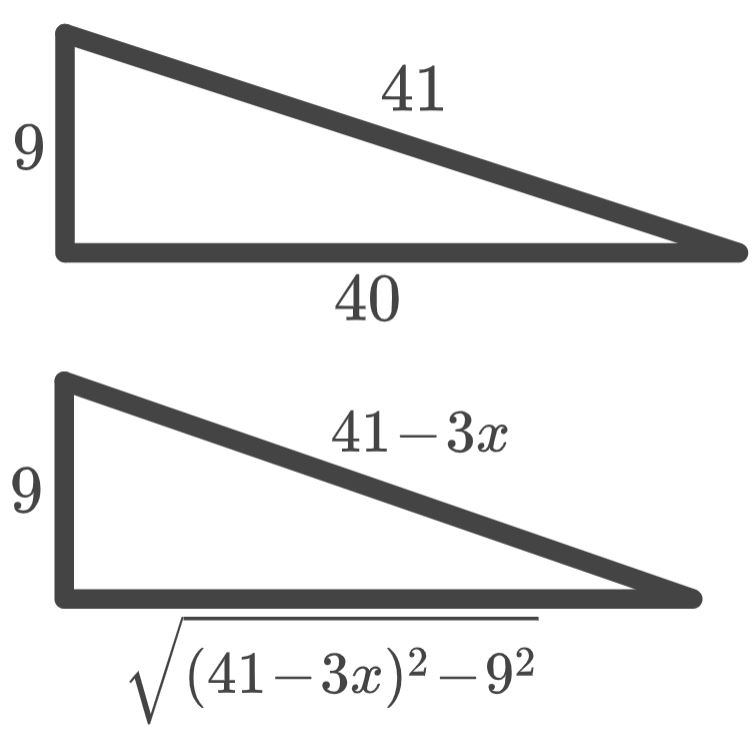
\includegraphics[width=\linewidth]{sol7}
        \end{figure}
    \end{minipage}
\end{minipage}
\smallskip\\Таким образом, мы получили зависимость координаты плота от времени: $$s(x) = \sqrt{1600 - 246x + 9x^2}.$$
Для того, чтобы найти скорость плота, найдём производную этого выражения (так как производная показывает скорость изменения величин).\\ Для этого используем цепное правило $\,(f(x) = \sqrt{x}$, $\,g(x) = 1600 - 246x + 9x^2$):\\
$s'(x) = \left(\sqrt{1600 - 246x + 9x^2}\right)' = \frac{1}{2\sqrt{1600 - 246x + 9x^2}} \cdot \left(-246 + 18x\right) = \frac{9x - 123}{\sqrt{1600 - 246x + 9x^2}}$.
Итак, мы нашли скорость плота в зависимости от времени $x$ (мин): $$s'(x) = v(x) = \frac{9x - 123}{\sqrt{1600 - 246x + 9x^2}}$$
Поскольку нам нужно найти скорость только в конкретный момент времени~--- вначале, когда расстояние от плота до берега равно 40 м, находим $v(0)$:\\ $\displaystyle v(0) = \frac{0 - 123}{\sqrt{1600}} = -\frac{123}{40} = -3\frac{3}{40} = -3{,}075$ м/мин.\\ Скорость получилась отрицательной, так как в нашей системе координат ось\\ направлена влево, поэтому ответ~--- $v = 3{,}075$ м/мин.}
{В этот момент времени скорость плота будет составлять $3{,}075$ м/мин.}{В задаче содержится прямоугольный треугольник~--- можно, пользуясь теоремой Пифагора, получить выражение для расстояния от плота до берега, и взяв производную получить скорость.}
\end{problem}

\begin{problem}{Дифференцирование сложной функции.}{10.5.9}{10A red переиграть числа}{(не лёгкая)}
{По двум улицам движутся к перекрёстку две машины с постоянными скоростями 40 км/ч и 50 км/ч. Считая, что улицы прямые и пересекаются под прямым углом, а также зная, что в некоторый момент времени машины находятся от перекрёстка на расстоянии 2 км и 3 км соответственно, определить, через какое время расстояние между машинами будет наименьшим.}
{Пусть с указанного некоторого момента времени прошло неизвестное время $t$. Тогда расстояние от первой машины до перекрёстка равно $|2 - 40t|$ км, а от второй машины до перекрёстка~--- $|3 - 50t|$ км.\\ Расстояние между двумя машинами может быть найдено по теореме Пифагора (причём независимо от того, проехала уже машина перекрёсток или нет): $$l(t) = \sqrt{(2 - 40t)^2 + (3 - 50t)^2} = \sqrt{4100t^2 - 460t + 13}.$$ Для нахождения минимума найдём ноль производной: \begin{multline*}
    l'(t) = \frac{1}{2\sqrt{4100t^2 - 460t + 13}}\cdot (8200t - 460) = 0 \;\Rightarrow\;\\
    \;\Rightarrow\; \frac{4100t - 230}{\sqrt{4100t^2 - 460t + 13}} = 0 \Rightarrow\; 4100t - 230 = 0 \;\Rightarrow\; t = \frac{23}{410}.
\end{multline*}
Понятно, что при очень большом $t$ расстояние между машинами будет увеличиваться, поэтому  найденное нами значение~--- точка минимума (для подкоренного выражения это вершина параболы с ветвями вверх). Итого, ответ: $t = \frac{23}{410}$ ч.}
{Расстояние между машинами будет наименьшим через $\frac{23}{410}$ часа.}{Составь выражение для расстояния между машинами в зависимости от времени и найди минимум этого выражения.}
\end{problem}

\begin{problem}{Дифференцирование сложной функции.}{10.5.9}{10A}{(лёгкая)}
{На параболе $y = x^2$ есть такая точка, расстояние от которой до точки $A = (2;\, \frac12)$ является наименьшим из всех возможных. Найти координаты этой точки.}
{Пусть $x$-координата искомой точки равна $x$. Тогда её $y$-координата равна $x^2$ (ведь она лежит на данной параболе и удовлетворяет уравнению $y = x^2$).
Итого, нужно найти наименьшее расстояние между точками $(2;\, \frac12)$ и $(x; \, x^2)$.\\
Расстояние между двумя точками может быть вычислено по теореме Пифагора: $l(x) = \sqrt{(x_1 - x_2)^2 + (y_1 - y_2)^2} = \sqrt{(x - 2)^2 + (x^2 - \frac12)^2} = \sqrt{x^4 - 4x + \frac{17}{4}}$.\\
Как мы и ожидали, расстояние является функцией от $x$.\\
Значит, мы можем найти минимум этой функции:
$$l'(x) = \frac{1}{2\sqrt{x^4 - 4x + \frac{17}{4}}} \cdot (4x^3 - 4) = 0 \;\Rightarrow\; x^3 - 1 = 0 \;\Rightarrow\; (x - 1)(x^2 + x + 1) = 0.$$
\vspace{-6mm}\\\begin{minipage}{\linewidth}
    \begin{minipage}{0.48\linewidth}
    Квадратное уравнение $x^2 + x + 1 = 0$\\ вещественных корней не имеет ($D = 1 - 4 < 0$), поэтому есть только одна критическая точка $x = 1$.\\ Следовательно, $y = 1^2 = 1$. Несложно убедиться, что это действительно минимум функции $l(x)$, а не максимум.
    \end{minipage}
    \hspace{0.02\linewidth}
    \begin{minipage}{0.50\linewidth}\begin{figure}[H] 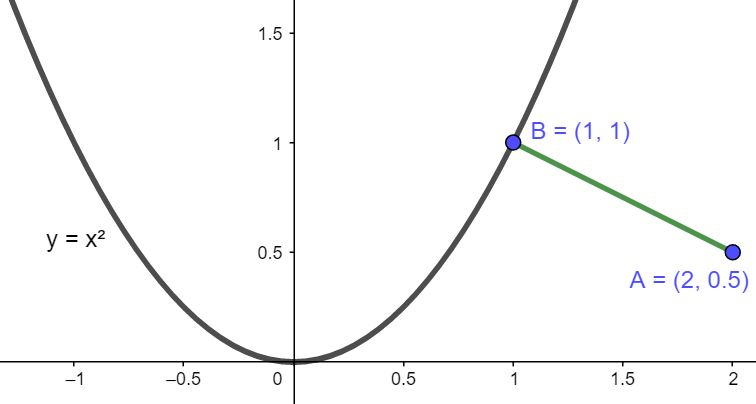
\includegraphics[width=\linewidth]{sol60}\end{figure}\end{minipage}\medskip
\end{minipage}
Построенный график можно увидеть на рисунке сверху.}
{Эта точка имеет координаты $(1; \, 1)$.\\
\textbf{Комментарий:} Можно было сразу искать минимум квадрата расстояния.\\ Единственное, как знаменатель производной $l'(x)$ влияет на рассуждения~--- мы должны убедиться, что подкоренное выражение положительно.\\ Но если это расстояние, то оно положительно, и проверку можно пропустить.}{Пусть точка имеет $x$-координату, равную $x$.\\ Чему тогда равно расстояние между двумя точками?}
\end{problem}

\begin{problem}{Дифференцирование сложной функции.}{10.5.9}{10A}{*}
{На параболе $y = x^2$ есть такая точка, расстояние от которой до точки $B = (6;\, 3)$ является наименьшим из всех возможных. Найти координаты этой точки.}
{НаписанноеРешение}
{ВерныйОтвет}{Подсказка}
\end{problem}

\begin{problem}{Уравнение касательной к графику функции.}{10.5.10}{10A}{(лёгкая)}
{При каких значениях параметра $b$ прямая $y = 3x + b$ является касательной к графику функции $y = \sqrt{x}$?}
{Если в некоторой точке $x_0$ к графику функции $f(x)$ провели касательную $l(x) = kx + d$, то в точке касания и функция, и касательная растут одинаково быстро (то есть, $f'(x_0) = k$). Найдем производную нашей функции $f(x) = \sqrt{x}$: $\,f'(x) = \frac{1}{2\sqrt{x}}$. Следовательно, $f'(x_0) = \frac{1}{2\sqrt{x_0}}$. У нашей прямой $k = 3$, откуда $\frac{1}{2\sqrt{x_0}} = 3 \;\Rightarrow\; 1 = 6\sqrt{x_0} \;\Rightarrow\; x_0 = \frac{1}{36}$. Значит, мы нашли абсциссу точки пересечения. Но тогда $\sqrt{\frac{1}{36}} = 3\cdot\frac{1}{36} + b \;\Rightarrow\; b = \frac16 - \frac{1}{12} = \frac{1}{12}$. Никаких других точек пересечения мы не нашли, есть только одно подходящее значение: $b = \frac{1}{12}$.}
{При $b = \frac{1}{12}$.}{Если две функции $f$ и $g$ касаются в точке $x_0$, то $f(x_0) = g(x_0)$ и $f'(x_0) = g'(x_0)$.}
\end{problem}

\begin{problem}{Уравнение касательной к графику функции.}{10.5.10}{10A}{*}
{Является ли прямая $y = 4x - 5$ касательной к графику функции $y = x^3 + x^2 - x - 2$? Если является, найти координаты точки касания.}
{Если функция $l(x)$ является касательной к $f(x)$, то как минимум эти две функции должны пересечься в некоторой точке касания $x_0$. Тогда $l(x_0) = y_0 = f(x_0)$ и получается, что $4x_0 - 5 = x_0^3 + x_0^2 - x_0 - 2$, откуда $x_0^3 + x_0^2 - 5x_0 + 3 = 0$.\smallskip\\ Решаем данное уравнение третьей степени: несложно увидеть, что $x_0 = 1$ является одним из решений. Тогда $x_0^3 + x_0^2 - 5x_0 + 3 = (x_0 - 1)(x_0^2 + 2x_0 - 3) = 0$. Квадратное уравнение решаем через дискриминант: $D = 4 + 12 = 16 \;\Rightarrow\; x_0 = \frac{-2\pm4}{2} = 1, -3$.\smallskip\\ Таким образом, или $x_0 = 1$, или $x_0 = -3$~--- в этих двух точках прямая имеет с функцией общую точку. Для того чтобы было касание, помимо этого нужно чтобы и функция, и касательная росли одинаково быстро (то есть, $f'(x_0) = l'(x_0)$).\smallskip\\ Находим производную нашей функции: $\,f'(x) = (x^3 + x^2 - x - 2)' = 3x^2 + 2x - 1$.\smallskip\\ Следовательно, $f'(1) = 3 + 2 - 1 = 4 = k$, в этой точке данная прямая является касательной. Во второй точке $f'(-3) = 3\cdot9 + 2\cdot(-3) - 1 = 20 \neq 4$, а значит, это просто вторая точка пересечения. Таким образом, точка касания~--- $x_0 = 1$. Находим $y_0$: $\,y_0 = 4x_0 - 5 = 4 - 5 = -1$.}
{Точка касания имеет координаты $(1, -1)$.}{Если две функции $f$ и $g$ касаются в точке $x_0$, то $f(x_0) = g(x_0)$ и $f'(x_0) = g'(x_0)$.}
\end{problem}

\begin{problem}{Уравнение касательной к графику функции.}{10.5.10}{10A}{(лёгкая)}
{Написать уравнение всех касательных к графику функции $y = x^3 - 2x + 7$,\\ параллельных прямой $y = x$.}
{Уравнение касательной к графику функции $f(x)$ в точке $x_0$ имеет вид $l(x) = f'(x_0)(x - x_0) + f(x_0)$. Как мы знаем, прямые $y_2 = k_1x + b_1$ и $y_2 = k_2x + b_2$ параллельны тогда и только тогда, когда $k_1 = k_2$.
\vspace{-4mm}\\\begin{minipage}{\linewidth}
    \begin{minipage}{0.35\linewidth}
    \vspace{1mm}
    Следовательно, должно быть выполнено уравнение $f'(x_0) = 1$. Вычислим производную в точке $x_0$: \vspace{-3mm}$$f'(x_0) = 3x_0^2 - 2.$$
    $3x_0^2 - 2 = 1 \;\Rightarrow\; 3x_0^2 = 3 \;\Rightarrow\; x_0 = \pm1$.\\ Таким образом, в этих двух точках касательная будет параллельна прямой $y = x$.\smallskip\\ Находим уравнения этих двух касательных: \\при $x_0 = 1$ получаем $l_1(x) = x - 1 + f(1) = x + 5$.\\ При $x_0 = -1$ получаем $l_2(x) = x + 1 + f(-1) = x + 9$.
    \end{minipage}
    \hspace{0.04\linewidth}
    \begin{minipage}{0.6\linewidth}\begin{figure}[H] 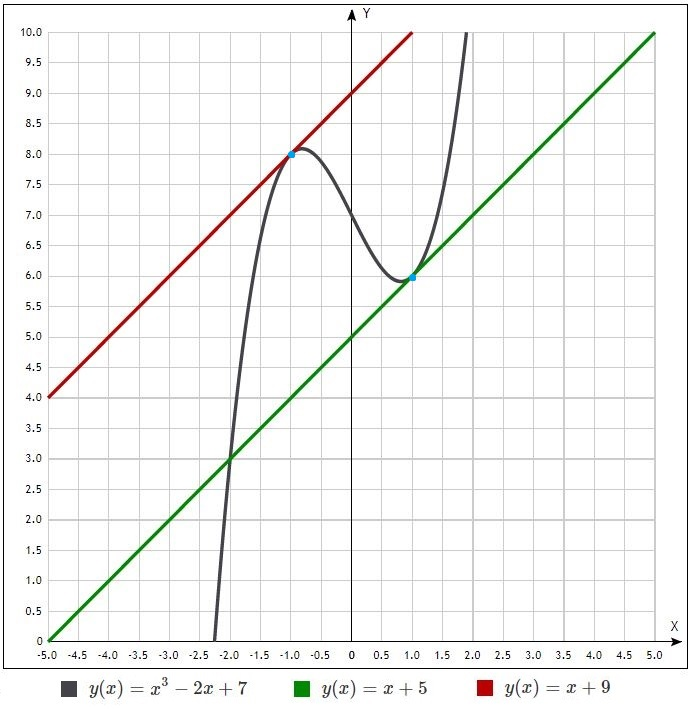
\includegraphics[width=\linewidth]{sol22}\end{figure}\end{minipage}
\end{minipage}}
{Касательных, параллельных прямой $y = x$, у функции $f(x) = x^3 - 2x + 7$ две~--- это $y = x + 5$ и $y = x + 9$.}{Чему должна быть равна производная функции $f(x)$ и в каких точках $x_0$ это выполнено?}
\end{problem}

\begin{problem}{Уравнение касательной к графику функции.}{10.5.10}{10A}{(лёгкая)}
{Показать, что параболы $y_1(x) = 3x^2 - 5x - 2$ и $y_2(x) = 2x^2 - x - 6$ имеют в их общей точке общую касательную. Найти уравнение этой касательной.}
{Утверждается, что общая точка у этих двух парабол есть, найдём её: $3x^2 - 5x - 2 = 2x^2 - x - 6 \;\Rightarrow\; x^2 - 4x + 4 = 0 \;\Rightarrow\; (x - 2)^2 = 0 \;\Rightarrow\; x = 2$.\\
Для нахождения тангенса угла наклона касательной (коэффициента $k$ прямой), вычислим производные в точке пересечения $x_0 = 2$ парабол $y_1(x)$ и $y_2(x)$:
\vspace{-4mm}\\\begin{minipage}{\linewidth}
    \begin{minipage}{0.35\linewidth}
    {\centering $\,y_1'(x) = 6x - 5 \;\Rightarrow\;$\\} {\centering $y_1'(2) = 12 - 5 = 7$.\medskip\\}
    {\centering $\,y_2'(x) = 4x - 1 \;\Rightarrow\;$\\}
    {\centering $y_2'(2) = 8 - 1 = 7$.\bigskip\\}
    Таким образом, данные параболы имеют ровно одну общую точку, $x = 2$, и в этой точке касательные к параболам параллельны, а значит, эти касательные совпадают.\smallskip\\ Уравнение этой касательной имеет вид $y = 7(x - 2) + y_1(2) = 7x - 14 + 0 = 7x - 14$.\medskip\\
    Касание парабол отображено на рисунке справа.
    \end{minipage}
    \hspace{0.04\linewidth}
    \begin{minipage}{0.6\linewidth}\begin{figure}[H] 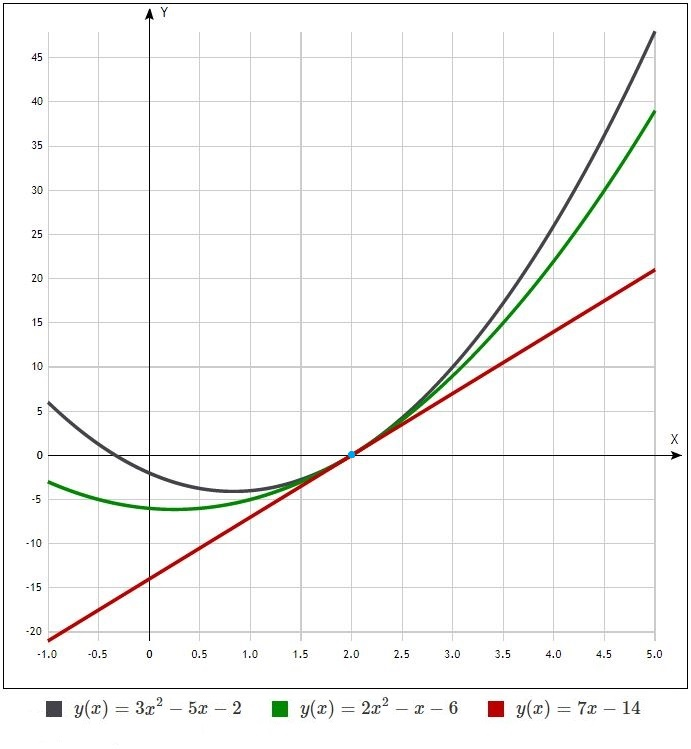
\includegraphics[width=\linewidth]{sol23}\end{figure}\end{minipage}
\end{minipage}\vspace{-4mm}\\}
{Параболы касаются в точке $(2; 0)$.\\ Уравнение касательной имеет вид $y = 7x - 14$.}{Какая общая точка этих двух парабол?}
\end{problem}

\begin{problem}{Уравнение касательной к графику функции.}{10.5.10}{10A}{(лёгкая)}
{Может ли касательная к гиперболе $y = \frac1x$ в какой-то точке $x$ образовывать острый угол с положительным направлением оси $Ox$?}
{Для касательной в точке $x$ тангенс угла наклона касательной $\tg \varphi = \\ = k = y'(x) = \left(\frac1x\right)' = -\frac{1}{x^2}$. Следовательно, $\tg \varphi < 0$ для любого значения $x \neq 0$.\smallskip\\ Это означает, что $\varphi \in(\frac{\pi}{2}; \pi)$. То есть возможны только тупые углы, острый угол с положительным направлением оси абсцисс получиться не может.}
{Нет, не может.}{Чему равен знак тангенса угла наклона касательной?}
\end{problem}

\begin{problem}{Уравнение касательной к графику функции.}{10.5.10}{10A}{(лёгкая)}
{Найти уравнение, которое задаёт прямую, перпендикулярную графику функции $y = x - x^3$ и имеющую с ним общую точку $(-1; 0)$.}
{НаписанноеРешение}
{ВерныйОтвет}{Подсказка}
\end{problem}

\begin{problem}{Уравнение касательной к графику функции.}{10.5.10}{10A}{(лёгкая)}
{Найти все значения $x$, при каждом из которых касательные к графикам функций $y = 3\cos 5x$ и $y = 5\cos 3x + 2$ в точках с абсциссой $x$ параллельны друг другу.}
{НаписанноеРешение}
{ВерныйОтвет}{Подсказка}
\end{problem}

\begin{problem}{Положительная, отрицательная, и нулевая производная.}{10.5.11}{10A red тут может вестись спор насчёт границ, но в ответе энивей интервал}{(лёгкая)}
{Найти интервал, на котором функция $f(x) = 3x^2 - 18x^3$ возрастает.}
{НаписанноеРешение}
{ВерныйОтвет}{Подсказка}
\end{problem}

\begin{problem}{Положительная, отрицательная, и нулевая производная.}{10.5.11}{10A}{*}
{Найти наименьшее и наибольшее значения функции $s(x) = 2\sin x + \sin 2x$ на отрезке $[0; \frac{3\pi}{2}]$.}
{Для нахождения локальных минимумов и максимумов надо выяснить \\промежутки возрастания и убывания функции $s(x)$. Находим производную:\\ $s'(x) = 2\cos x + 2\cos 2x = 2\cdot(\cos x + 2\cos^2 x - 1) = 2\cdot(2\cos^2 x + \cos x - 1)$.\smallskip\\
Решаем неравенство $s'(x) > 0$ методом интервалов: для этого сначала решим уравнение $s'(x) = 0$: $s'(x) = 2\cdot(2\cos^2 x + \cos x - 1) = 0 \;\Rightarrow\;$ (делаем замену $t = \cos x$) $\;\Rightarrow\; 2t^2 + t - 1 = 0 \;\Rightarrow\; (2t - 1)(t + 1) = 0 \;\Rightarrow\; t = \frac12$ или $t = -1$.\smallskip\\
Решая квадратное неравенство, получаем что $s'(x) < 0$ при $-1 < t < \frac12$ и больше 0 при $t \not\in (-1;\, \frac12)$. Теперь, учитывая, что $t = \cos x$, надо решить тригонометрические уравнения $\cos x = -1$ и $\cos x = \frac12$:\\
$\cos x = -1 \;\Rightarrow\; x = \pi + 2\pi n$, $\,n \in \mathbb{Z}$.\hfill $\cos x = \frac12 \;\Rightarrow\; x = \pm\frac{\pi}{3} + 2\pi k$, $\,k \in \mathbb{Z}$.\smallskip\\
Функция $s(x)$, также как и её производная, периодична с периодом $T = 2\pi$.\\ Поэтому рассмотрим отрезок $[0; 2\pi]$. На $[0; \frac{\pi}{3})$ функция $s(x)$ возрастает ($s'(x) > 0$).\\ На обоих промежутках $(\frac{\pi}{3}; \pi)$ и $(\pi; \frac{5\pi}{3})$ функция $s(x)$ убывает ($s'(x) < 0$), и поэтому, так как данная функция непрерывна, все точки вида $x = \pi + 2\pi n,\,n\in \mathbb{Z}$ являются точками перегиба. На интервале $(\frac{5\pi}{3}; 2\pi]$ $s(x)$ снова возрастает, $s'(x) > 0$.\smallskip\\ Следовательно, так как нам нужно рассмотреть лишь отрезок $[0; \frac{3\pi}{2}]$, и $\frac{3\pi}{2} < \frac{5\pi}{3}$, то минимум достигается в точке $x = 0$ или $x = \frac{3\pi}{2}$, а максимум~--- в точке $x = \frac{\pi}{3}$.\smallskip\\ Находим значения во всех упомянутых точках:\\
$s(0) = 2\sin 0 + \sin 2\cdot0 = 0$; $\;s(\frac{3\pi}{2}) = 2\sin\frac{3\pi}{2} + \sin 3\pi = 2\cdot (-1) + 0 = -2$. $s(\frac{\pi}{3}) = 2\sin\frac{\pi}{3} + \sin \frac{2\pi}{3} = 2\cdot\frac{\sqrt{3}}{2} + \frac{\sqrt{3}}{2} = \frac{3\sqrt{3}}{2}$. Таким образом, на данном отрезке наименьшее значение функции достигается в $x = \frac{3\pi}{2}$ и равно $s(\frac{3\pi}{2}) = -2$, а наибольшее значение достигается в точке $x = \frac{\pi}{3}$ и равно $s(\frac{\pi}{3}) = \frac{3\sqrt{3}}{2} \approx 2{,}6$.}
{Наибольшее значение функции $s(x)$ на отрезке $[0; \frac{3\pi}{2}]$ равно $s(\frac{\pi}{3}) = \frac{3\sqrt{3}}{2}$, наименьшее значение равно $s(\frac{3\pi}{2}) = -2$.
\vspace{-4mm}\\\begin{minipage}{\linewidth}
    \begin{minipage}{0.42\linewidth}
    График функции $s(x)$ (не только на этом отрезке) изображён на рисунке справа. Видно, что данная функция является периодической с периодом $T = 2\pi$ и амплитудой $A = \frac{3\sqrt{3}}{2}$, однако ведёт себя не так как функция $f(x) = A\sin (kx + \varphi_0)$ в точках вида $x = \pi + 2\pi n$, $\,n \in \mathbb{Z}$.\medskip\\ Говоря научно, у функции $s(x)$ все точки вида $x = 2\pi k$, $\,k \in \mathbb{Z}$~--- корни, имеющие кратность 1, в то время как точки $x = \pi + 2\pi n$, $\,n \in \mathbb{Z}$ это корни, имеющие кратность 3.
    \end{minipage}
    \hspace{0.03\linewidth}
    \begin{minipage}{0.54\linewidth}\begin{figure}[H] 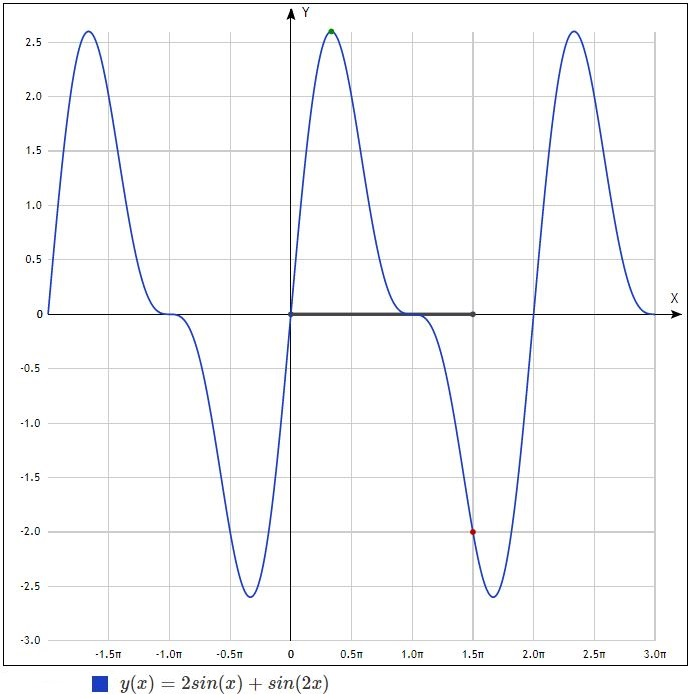
\includegraphics[width=\linewidth]{sol40}\end{figure}\end{minipage}
\end{minipage}}{Как и всегда в задачах на нахождение минимума/максимума, нужно взять производную и найти промежутки возрастания и убывания функции $s(x)$.}
\end{problem}

\begin{problem}{Положительная, отрицательная, и нулевая производная.}{10.5.11}{10A}{*}
{Дана функция $f(x) = |x^3 - 12x + r|$, зависящая от параметра $r$.\\ Найти её особые точки и их тип (локальный минимум / максимум).\\ Вычислить сумму значений функции в этих особых точках, то есть величину $f(x_1) + f(x_2) + \ldots + f(x_k)$, если известно, что $r \in [-15; 15]$.}
{Данная задача по сложности тянет на олимпиадную.\\ Поэтому решение будет отчасти в стиле <<как до такого додуматься>>.\smallskip\\
Мысль №1: поскольку мы знаем, что модуль может либо поменять знак, либо не поменять, получается, что нашу функцию можно записать как кусочнозаданную: $f(x) = \left\{\begin{aligned}
x^3 - 12x + r, \text{ если } x \in D\\
-x^3 + 12x - r, \text{ если } x \notin D,
\end{aligned}\right.$ $\quad$\parbox{9cm}{где $D$~--- множество $x$, являющихся \\решением неравенства $x^3 - 12x + r > 0$.}\\
Это довольно серьёзное продвижение в решении, поскольку для кусочнозаданной функции уже можно вычислять производную. Однако, мы всё ещё не нашли множество $D$. Отсюда появляется идея для следующего шага.\smallskip\\
Мысль №2: надо провести исследование функции $g(x) = x^3 - 12x + r$ с параметром $r$. Для решения неравенства $g(x) > 0$ было бы неплохо явно найти корни, но поскольку это не представляется возможным, попробуем найти что-нибудь ещё.
\smallskip\\
Мысль №3: Мы можем найти производную. $g'(x) = 3x^2 - 12$.\\ Мы видим, что производная не зависит от параметра $r$! Это значит, что мы на верном пути и можем сделать какие-то выводы для любых значений параметра.\\ Найдём нули производной и промежутки возрастания и убывания функции $g(x)$. $g'(x) = 3(x^2 - 4) = 0 \;\Rightarrow\; x^2 - 4 = 0 \;\Rightarrow\; x = \pm 2$. Это означает, что функция $g(x)$ возрастает при $x \in (-\infty; -2) \cup (2; +\infty)$ и убывает при $x \in (-2; 2)$, поэтому $x = -2$~--- точка локального максимума, а $x = 2$~--- точка локального минимума. \\ Найдём значения функции $g(x)$ в точках $2$ и $-2$: $g(-2) = (-2)^3 - 12\cdot(-2) + r = -8 + 24 + r = r + 16$, $\,g(2) = 2^3 - 12\cdot2 + r = r - 16$.\\ Итого, локальный максимум~--- $r + 16$, локальный минимум~--- $r - 16$.\smallskip\\
Мысль №4: для решения задачи нужно использовать всё, что нам дано. Пока мы никак не использовали условие, что $r \in [-15; 15]$. А ведь этот интервал даёт конкретную информацию: при таком $r$ значение $g(-2) = r + 16$ гарантированно больше 0, а $g(2) = r - 16$ гарантированно меньше 0. Следовательно, для любых значений $r \in [-15; 15]$ уравнение $g(x) = 0$ имеет ровно 3 решения $x_1$, $x_2$, $x_3$.\\
Мы нашли $D$, $D = (x_1; x_2)\cup(x_3; +\infty)$ (подразумевается, что $x_1 < x_2 < x_3$).\smallskip\\
Мысль №5: мы можем представить, как выглядит график функции $f(x)$:\\ многочлен третьей степени с 3 корнями, отражённый относительно оси абсцисс там, где его значение отрицательно (на интервалах $(-\infty; x_1)$ и $(x_2; x_3)$).\\ Производную также можно найти явно: \\ $f'(x) = \left\{\begin{aligned}
3x^2 - 12, &\text{ если } x \in (x_1; x_2) \cup (x_3; +\infty)\\
-3x^2 + 12, &\text{ если } x \in (-\infty; x_1) \cup (x_2; x_3),
\end{aligned}\right.$ $\quad$\parbox{6cm}{а в точках $x_1$, $x_2$, $x_3$ производная не определена.}\\
\textit{Комментарий:} Производная для $f(x)$ в точке $x_i$ была бы определена, если бы для этого $i \in \{1, 2, 3\}$ было бы выполнено $3x_i^2 - 12 = -3x_i^2 + 12 \Leftrightarrow 6x_i^2 = 24 \Leftrightarrow$ \\ $\Leftrightarrow x_i^2 = 4 \Leftrightarrow x_i = \pm2$. Но мы знаем, что $x_1\in(-\infty; -2)$, $x_2 \in (-2; 2)$, $x_3 \in (2; +\infty)$, поэтому такое невозможно.\smallskip\\ Значит, мы уже нашли все критические точки функции $f(x)$~--- это $-2$ и 2.\\ Значения в них до отражения были равны $r + 16 > 0$ и $r - 16 < 0$.\\ После отражения локальный минимум станет локальным максимумом, второе значение поменяет знак, и в результате $f(-2) = r + 16$, $f(2) = -(r - 16) = 16 - r$.\\ Находим то, что требовалось: $f(-2) + f(2) = r + 16 + 16 - r = 32$.}
{Функция $f$ независимо от $r$ имеет две критических точки, $x = -2$ и $x = 2$. При данных ограничениях на $r$, обе критических точки будут локальными максимумами, а сумма значений функции в них будет равна 32.\\
\textit{Комментарий:} отмечу, что только при $r \in (-16; 16)$ локальный минимум и максимум имеют разные знаки. Если взять $r \notin [-16; 16]$, то в итоге знаки будут одинаковы, и $f(-2) + f(2)$ будет получаться равным $|r + 16 + r - 16| = |2r|$.\\
Построенный график можно посмотреть \href{https://tinyurl.com/y3q832ug}{\textbf{здесь}}.
}{Надо раскрыть модуль двумя способами, несмотря на то, что границы интервала(ов) неизвестны. Провести исследование нужной функции с помощью производной и максимально использовать данное на $r$ ограничение.}
\end{problem}

\begin{problem}{Положительная, отрицательная, и нулевая производная.}{10.5.11}{10A}{*}
{Функция $B(x)$ задана кусочно: $B(x) = \left
\{\begin{aligned}
    -x^2 - 4x + 3, \text{ если } x &< -1\\
    3x^{10} + 7, \quad \!\text{ если } -1 &\leqslant x \leqslant 1\\
    -x^2 + 4x + 3, \text{ если } 1 &< x.
\end{aligned}\right.$\\
Найти минимумы и максимумы функции $B(x)$.}
{Вычислим производную $B'(x)$ (которая также будет кусочнозаданной функцией) и найдём промежутки возрастания и убывания, решив неравенство $B'(x) > 0$.\vspace{-4mm}\\
$B'(x) = \left\{\begin{aligned}
    -2x - 4, \text{ если } x &< -1\\
    30x^9, \,\text{ если } -1 &\leqslant x \leqslant 1\\
    -2x + 4, \text{ если } 1 &< x.
\end{aligned}\right.\quad$ \parbox{9cm}{Находим критические точки: при $x < -1$ есть одна критическая точка $x = -2$, при $x > 1$ есть критическая точка $x = 2$, и на центральном интервале также есть единственная критическая точка $x = 0$.}
\vspace{-2mm}\\\begin{minipage}{\linewidth}
    \begin{minipage}{0.42\linewidth}
    Расстановка знаков производной даёт результат, изображённый на рисунке справа: 
    \end{minipage}
    \hspace{0.03\linewidth}
    \begin{minipage}{0.54\linewidth}\begin{figure}[H] 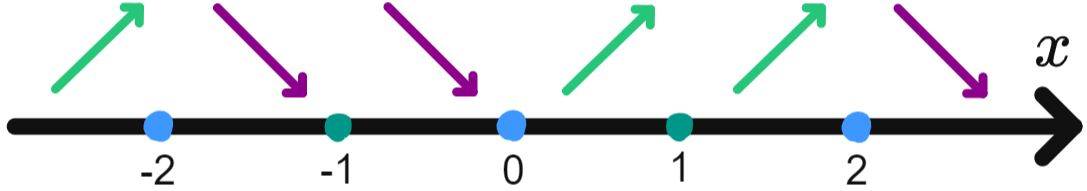
\includegraphics[width=\linewidth]{sol41}\end{figure}\end{minipage}
\end{minipage}
Конечно, хочется сразу сказать, что максимумы функции $B(x)$ достигаются в точках $x = \pm 2$, а минимум~--- в точке $x = 0$. Однако будем внимательны!\smallskip\\ В самом деле, функция $B(x)$~--- кусочнозаданная. А значит, могут быть точки разрыва, в результате чего возможны примеры, аналогичные гиперболе $f(x) = \frac1x$ (убывает и левее 0, и правее 0, но $f(-1) < f(1)$). Поэтому найдём значения во всех пяти точках: $B(-2) = -(-2)^2 - 4(-2) + 3 = 7$, $\:B(-1) = 3\cdot(-1)^{10} + 7 = 10$, $B(0) = 3\cdot0 + 7 = 7$, $\;B(1) = 3\cdot1^{10} + 7 = 10$, $\;B(2) = -2^2 + 4\cdot2 + 3 = 7$.
\vspace{-4mm}\\\begin{minipage}{\linewidth}
    \begin{minipage}{0.42\linewidth}
    Таким образом, точки $x = \pm2$~--- точки локального максимума, точка $x = 0$~--- точка локального минимума, но максимальное значение функции равно $B(-1) = B(1) = 10$, а наименьшее значение у функции $B(x)$ отсутствует (левая парабола и правая парабола уходят в минус бесконечность)\medskip\\
    Для прояснения ситуации, график функции $B(x)$ изображён на рисунке справа:
    \end{minipage}
    \hspace{0.03\linewidth}
    \begin{minipage}{0.54\linewidth}\begin{figure}[H] 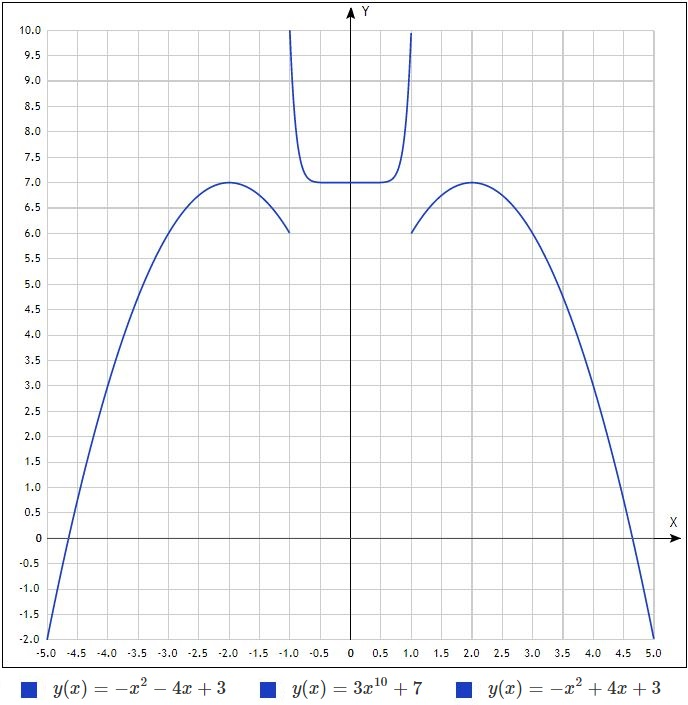
\includegraphics[width=\linewidth]{sol42}\end{figure}\end{minipage}
\end{minipage}}
{Функция $B(x)$ имеет локальные максимумы в точках $x = -2$ и $x = 2$, и локальный минимум в точке $x = 0$. Однако, $B(-2) = B(0) = B(2) = 7$, а максимальное значение из-за наличия двух точек разрыва достигается в точках $x = -1$ и $x = 1$ и равно 10. Минимального значения нет.}{Функция $B(x)$ имеет точки разрыва.}
\end{problem}

\begin{problem}{Положительная, отрицательная, и нулевая производная.}{10.5.11}{10A}{*}
{Решить уравнение $4x + \pi\sin x = 3\pi$ и показать, что других решений нет.}
{После недолгих размышлений можно заметить, что $x = \pi$ является корнем: действительно, $4\pi + \pi\sin \pi = 4\pi - \pi = 3\pi$.\\ Интуиция подсказывает, что раз слагаемое $4x$ неограниченно растёт, а $\pi\sin x$ заперто в полосе $[-\pi; \pi]$, решений не должно быть много.\\ Для того чтобы исследовать скорость роста, взглянем на производную левой\\ части уравнения: $(4x + \pi\sin x)' = 4 + \pi \cos x$.\smallskip\\
\textit{Факт, решающий задачу:} $4 + \pi \cos x > 0 \;\;\forall x$ (очевидно, так как $|\pi| < |4|$).\\ Это означает, что производная положительна для любых $x$, то есть левая часть уравнения растёт на всём $\mathbb{R}$. Значит, мы решаем уравнение вида $f(x) = a$, где $f$~--- монотонно возрастающая функция. Поэтому корней не может быть больше одного, но один корень мы уже нашли~--- это $x = 4\pi$.\\ Следовательно, это и есть ответ, а других корней попросту нет.}
{Уравнение $4x + \pi\sin x = 3\pi$ имеет только один корень: $x = 4\pi$.}{Можно угадать один корень и показать, что левая часть уравнения~--- монотонная функция.}
\end{problem}

\begin{problem}{Построение графиков не типичных функций.}{10.5.12}{10A}{(лёгкая)}
{Провести полное исследование функции $f(x) = x^3 - 12x$, нарисовать её график.}
{НаписанноеРешение}
{ВерныйОтвет}{Подсказка}
\end{problem}

\begin{problem}{Построение графиков не типичных функций.}{10.5.12}{10A}{(лёгкая)}
{Провести полное исследование функции $h(x) = \displaystyle x^5 - x^3 - 2x$, нарисовать её график.

}
{Функция $h(x)$ является многочленом пятой степени, поэтому область определения $D(h)$~--- $\mathbb{R}$, везде на котором $h(x)$ непрерывна.\smallskip\\
Функция $h(x)$ является нечётной (так как у всех мономов, входящих в $h(x)$,\\ степень нечётна) $\;\Rightarrow\;$ график $h(x)$ центрально симметричен относительно нуля.\smallskip\\
Точек разрыва и вертикальных асимптот нет.\smallskip\\
Найдём точки пересечения $h(x)$ с осью абсцисс, решив уравнение $x^5 - x^3 - 2x = 0$:\\
$x^5 - x^3 - 2x = 0 \;\Rightarrow\; x(x^4 - x^2 - 2) = 0 \;\Rightarrow\; x(x^2 - 2)(x^2 + 1) = 0 \;\Rightarrow\; x = 0; \pm\sqrt{2}$.\smallskip\\
Поскольку $h(x) = x(x - \sqrt{2})(x + \sqrt{2})(x^2 + 1)$, то согласно методу интервалов, \\$h(x) > 0$ при $x \in (-\sqrt{2}; 0) \cup (\sqrt{2}; +\infty)\,$ и $\,h(x) < 0$ при $x \in (-\infty; -\sqrt{2}) \cup (0; \sqrt{2}).$\smallskip\\
Найдем критические точки функции $h(x)$, решив уравнение $h'(x) = 0$:\\ $h'(x) = 5x^4 - 3x^2 - 2 = 0 \;\Rightarrow\; (x^2 - 1)(5x^2 + 2) = 0 \;\Rightarrow\; x = \pm 1$.\smallskip\\
Теперь найдём промежутки возрастания и убывания функции $h(x)$:\\ $h'(x) = (x - 1)(x + 1)(5x^2 + 2)$, поэтому согласно методу интервалов, $h(x)$ возрастает на $(-\infty; -1) \cup (1; +\infty)$ ($h'(x) > 0$) и убывает на $(-1; 1)$ ($h'(x) < 0$).\\
\begin{minipage}{\linewidth}
    \begin{minipage}{0.39\linewidth}
Таким образом, функция $h(x)$ имеет две критические точки, $x = -1$ и $x = 1$.\smallskip\\
Учитывая знаки производной, в первой достигается локальный максимум ($h(-1) = 2$), а во второй~--- локальный минимум ($h(1) = -2$).\medskip\\
Горизонтальных и наклонных асимптот у функции $h(x)$ нет: поскольку $h(x)$~--- многочлен нечётной степени, $E(f) = \mathbb{R}$.\medskip\\
Построенный график изображён на рисунке справа:
    \end{minipage}
    \hspace{0.03\linewidth}
    \begin{minipage}{0.58\linewidth}\begin{figure}[H] 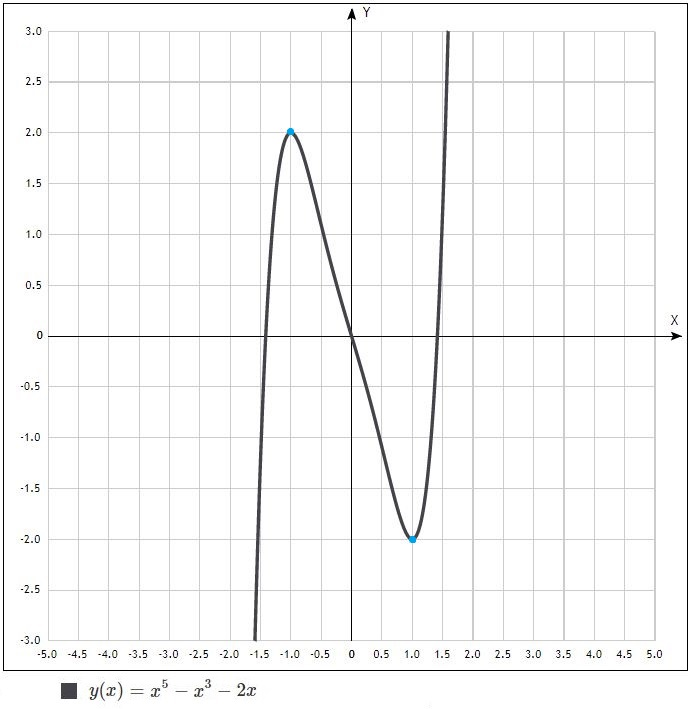
\includegraphics[width=\linewidth]{sol24}\end{figure}\end{minipage}
\end{minipage}\vspace{-4mm}}
{См. график.}{Выполнить все действия по схеме полного исследования функции.}
\end{problem}

\begin{problem}{Построение графиков не типичных функций.}{10.5.12}{10A}{(лёгкая)}
{Провести полное исследование функции $g(x) = \displaystyle \frac{x^2}{4x^2 - 1}$, нарисовать её график.}
{НаписанноеРешение}
{ВерныйОтвет}{Подсказка}
\end{problem}

\begin{problem}{Построение графиков не типичных функций.}{10.5.12}{10A}{(лёгкая)}
{Провести полное исследование функции $s(x) = \displaystyle \frac{x}{x^2 - 1}$, нарисовать её график.}
{НаписанноеРешение}
{ВерныйОтвет}{Подсказка}
\end{problem}

\begin{problem}{Построение графиков не типичных функций.}{10.5.12}{10A}{(лёгкая)}
{Провести полное исследование функции $m(x) = \displaystyle \frac{x^3}{x^2 - 4}$, нарисовать её график.}
{Область определения функции $m(x)$~--- $D(m) = \mathbb{R}\backslash\{-2, 2\}$.\smallskip\\
Функция $m(x)$ является нечётной, что означает наличие у графика данной функции центральной симметрии относительно начала координат.\smallskip\\
Точки $x = \pm 2$ являются точками разрыва $m(x)$. Проверяем наличие асимптот: $\lim\limits_{x\to-2-0}\displaystyle \frac{x^3}{x^2 - 4} = -\lim\limits_{x\to 2+0}\displaystyle \frac{x^3}{x^2 - 4} = -\infty. \quad \lim\limits_{x\to-2+0}\displaystyle \frac{x^3}{x^2 - 4} = -\lim\limits_{x\to 2-0}\displaystyle \frac{x^3}{x^2 - 4} = +\infty$.\smallskip\\
Поэтому функция $m(x)$ меняет знак в обеих точках разрыва и имеет там вертикальные асимптоты $x = -2$ и $x = 2$. \smallskip\\
Находим точки пересечения $m(x)$ с осью абсцисс: $m(x) = \displaystyle \frac{x^3}{x^2 - 4} = 0 \;\Rightarrow\; x = 0$.\smallskip\\
Согласно методу интервалов, $m(x) > 0$ при $x \in (-2; 0) \cup (2; +\infty)\,$ и\\ $\,m(x) < 0$ при $x \in (-\infty; -2) \cup (0; 2).$ \smallskip\\
Найдем критические точки функции $m(x)$, решив уравнение $m'(x) = 0$:\\ $\displaystyle m'(x) = \left(\frac{x^3}{x^2 - 4}\right)' = \frac{3x^2 \cdot (x^2 - 4) - x^3 \cdot 2x}{(x^2 - 4)^2} = \frac{x^4 - 12x^2}{(x^2 - 4)^2} = \frac{x^2(x^2 - 12)}{(x^2 - 4)^2} = 0\;\Rightarrow\; x^2(x^2 - 12) = 0 \;\Rightarrow\; x = 0; \:x = \pm 2\sqrt{3}$.\\ Таким образом, $m(x)$ имеет три критических точки: $x = 0$ и $x = \pm2\sqrt{3}$.\smallskip\\
Теперь найдём промежутки возрастания и убывания:\\ $\displaystyle m'(x) \!=\! \frac{x^2(x - 2\sqrt3)(x + 2\sqrt3)}{(x - 2)^2 \cdot (x + 2)^2}$, поэтому, согласно методу интервалов,\\ $m(x)$ возрастает на $(-\infty; -2\sqrt{3}) \cup (2\sqrt{3}; +\infty)\;$ ($m'(x) > 0$) и \\убывает на $(-2\sqrt{3}; -2) \cup (-2; 0) \cup (0; 2) \cup (2; 2\sqrt{3})\;$ ($m'(x) < 0$).\smallskip\\
Учитывая знаки производной, в первой точке достигается локальный максимум: $m(-2\sqrt{3}) = \frac{(-2\sqrt{3})^3}{(-2\sqrt{3})^2 - 4} = -\frac{24\sqrt{3}}{12 - 4} = -3\sqrt{3}$. Во второй точке $x = 0$~--- перегиб. В третьей же точке получается локальный минимум: $m(2\sqrt{3}) = \frac{(2\sqrt{3})^3}{(2\sqrt{3})^2 - 4} = \frac{24\sqrt{3}}{12 - 4} = 3\sqrt{3}$.\vspace{-4mm}\\
\begin{minipage}{\linewidth}
    \begin{minipage}{0.41\linewidth}
Проверим наличие горизонтальных/наклонных асимптот у $m(x)$, сначала находим $k$:\\ $k = \displaystyle \!\!\lim\limits_{x\to\pm\infty}\!\!\frac{m(x)}{x} = \!\!\lim\limits_{x\to\pm\infty}\!\frac{x^2}{x^2 - 4} = 1.$\medskip\\ Теперь $b$: $\,\displaystyle b = \!\!\lim\limits_{x\to\pm\infty}(m(x) - kx) =$\\ $\displaystyle = \lim\limits_{x\to\pm\infty}\!\,\left(\frac{x^3}{x^2 - 4} - x\right) = \lim\limits_{x\to\pm\infty}\!\,\!\left(\frac{4x}{x^2 - 4}\right) = 0$.\smallskip\\ Поэтому прямая $y = x$ является наклонной асимптотой.\bigskip\\
График функции $m(x) = \frac{x^3}{x^2 - 4}$ изображён на рисунке справа:
    \end{minipage}
    \hspace{0.02\linewidth}
    \begin{minipage}{0.57\linewidth}\begin{figure}[H] 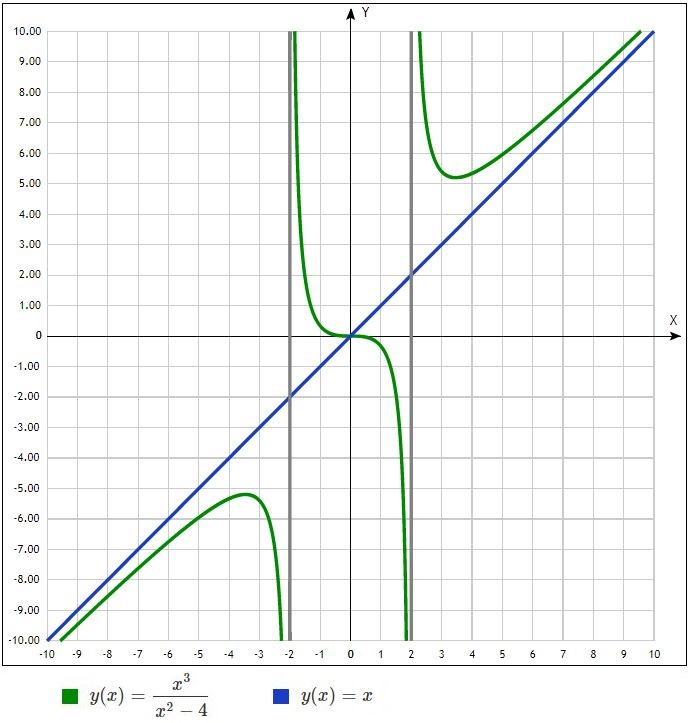
\includegraphics[width=\linewidth]{sol43}\end{figure}\end{minipage}
\end{minipage}\vspace{-9mm}}
{См. график.}{Выполнить все действия по схеме полного исследования функции.}
\end{problem}

\begin{problem}{Построение графиков не типичных функций.}{10.5.12}{10A red плохой текст: наличие асимптот надо проверять пределом}{(лёгкая)}
{Провести полное исследование функции $u(x) = \displaystyle \frac{x^3 - 1}{4x^2}$, нарисовать её график.}
{Область определения функции $u(x)$~--- $D(u) = \mathbb{R}\backslash\{0\}$.\smallskip\\
Функция $u(x)$ не является ни чётной, ни нечётной.\smallskip\\
Точка $x = 0$ является точкой разрыва $u(x)$, поэтому $x = 0$~--- вертикальная асимптота. Более того, так как $\lim\limits_{x\to\pm0}\displaystyle \frac{x^3 - 1}{4x^2} = \lim\limits_{x\to\pm0}\displaystyle \left(\frac{x}{4} - \frac{1}{4x^2}\!\right) = 0 -\infty = -\infty$, функция не меняет знак в этой точке. \smallskip\\
Найдём все точки пересечения $u(x)$ с осью абсцисс: $u(x) = \displaystyle \frac{x^3 - 1}{4x^2} = 0 \;\Rightarrow\; x^3 - 1 = 0 \;\Rightarrow\; (x - 1)(x^2 + x + 1) = 0 \;\Rightarrow\;x = 1$.\smallskip\\
Согласно методу интервалов, $u(x) > 0$ при $x \in (1; +\infty)\,$ и\\ $\,u(x) < 0$ при $x \in (-\infty; 0) \cup (0; 1).$ \smallskip\\
Найдем критические точки функции $u(x)$, решив уравнение $u'(x) = 0$:\\ $\displaystyle u'(x) = \left(\frac{x^3 - 1}{4x^2}\right)' = \frac{3x^2 \cdot 4x^2 - (x^3 - 1) \cdot 8x}{(4x^2)^2} = \frac{4x^4 + 8x}{16x^4} = \frac{x^3 + 2}{4x^3} = 0\;\Rightarrow\; x^3 + 2 = 0 \;\Rightarrow\; x = -\sqrt[3]{2}$.\smallskip\\
Теперь найдём промежутки возрастания и убывания:\\ $\displaystyle u'(x) \!=\! \frac{x^3 + 2}{4x^3}$, поэтому согласно методу интервалов, $u(x)$ убывает на $(-\sqrt[3]{2}; 0)$ ($u'(x) < 0$) и возрастает на $(-\infty; -\sqrt[3]{2}) \cup (0; +\infty)$ ($u'(x) > 0$).\smallskip\\
Таким образом, $u(x)$ имеет только одну критическую точку, $x = -\sqrt[3]{2}$.\\
Учитывая знаки производной, в этой точке достигается локальный максимум ($u(-\sqrt[3]{2}) = \frac{-2-1}{4\cdot\sqrt[3]{4}} = -\frac{3\sqrt[3]{2}}{8}$).\vspace{-8mm}\\
\begin{minipage}{\linewidth}
    \begin{minipage}{0.39\linewidth}
Проверим наличие горизонтальных/наклонных асимптот у $u(x)$, сначала находим $k$:\\ $k = \displaystyle \!\!\lim\limits_{x\to\pm\infty}\!\!\frac{u(x)}{x} = \!\!\lim\limits_{x\to\pm\infty}\!\frac{x^3 - 1}{4x^3} = \frac14$\medskip\\ Теперь $b$: $\,\displaystyle b = \!\!\lim\limits_{x\to\pm\infty}(u(x) - kx) =$\\ $\displaystyle = \lim\limits_{x\to\pm\infty}\!\,\left(\frac{x^3 - 1}{4x^2} - \frac{1}{4}x\right) = \lim\limits_{x\to\pm\infty}\!\,\!\left(-\frac{1}{4x^2}\right) = 0$.\smallskip\\ Поэтому прямая $y = \frac{x}{4}$ является наклонной асимптотой.\bigskip\\
График функции $u(x) = \frac{x^3 - 1}{4x^2}$ изображён на рисунке справа:
    \end{minipage}
    \hspace{0.03\linewidth}
    \begin{minipage}{0.58\linewidth}\begin{figure}[H] 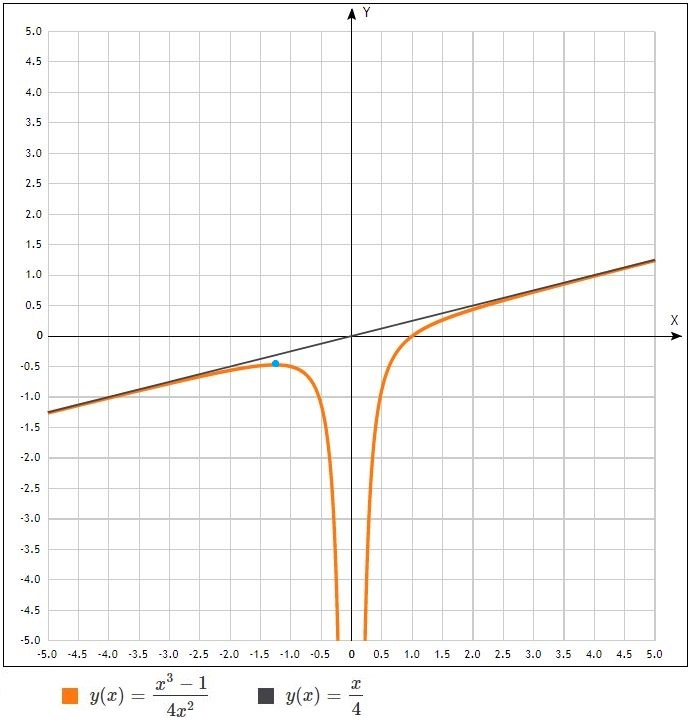
\includegraphics[width=\linewidth]{sol26}\end{figure}\end{minipage}
\end{minipage}\vspace{-6mm}}
{См. график.}{Выполнить все действия по схеме полного исследования функции.}
\end{problem}

\begin{problem}{Построение графиков не типичных функций.}{10.5.12}{10A}{(лёгкая)}
{Провести полное исследование функции $g(x) = \displaystyle \frac{2x}{x^2 + 4}$, нарисовать её график.}
{Функция $g(x)$ определена и непрерывна на всей числовой прямой (знаменатель дроби нигде не обращается в 0), поэтому область определения $D(g) = \mathbb{R}$.\smallskip\\
Функция $g(x)$ является нечётной. Действительно, $g(-x) = \displaystyle \frac{2\cdot(-x)}{(-x)^2 + 4} = -\frac{2x}{x^2 + 4}$, следовательно её график симметричен относительно начала координат.\smallskip\\
Точек разрыва у $g(x)$ нет, поэтому нет и вертикальных асимптот.\smallskip\\
Очевидно, что точка пересечения у $g(x)$ с осью абсцисс только одна~--- это $x = 0$ (дробь может быть равна нулю только если числитель равен нулю).\smallskip\\
Согласно методу интервалов, $g(x) > 0$ при $x > 0\,$ и $\,g(x) < 0$ при $x < 0.$ \smallskip\\
Найдем критические точки функции $g(x)$, решив уравнение $g'(x) = 0$:\\ $\displaystyle g'(x) = \left(\frac{2x}{x^2 + 4}\right)' = \frac{2\cdot(x^2 + 4) - 2x\cdot2x}{(x^2 + 4)^2} = \frac{8 - 2x^2}{(x^2 + 4)^2} = \frac{2(2 - x)(2 + x)}{(x^2 + 4)^2} = 0\;\Rightarrow\; (2 - x)(2 + x) = 0 \;\Rightarrow\; x = -2;\, 2$.\smallskip\\
Теперь найдём промежутки возрастания и убывания:\\ $\displaystyle g'(x) = \frac{2(2 - x)(2 + x)}{(x^2 + 4)^2}$, поэтому согласно методу интервалов, $g(x)$ убывает на $(-\infty; -2) \cup (2; +\infty)$ ($g'(x) < 0$) и возрастает на $(-2; 2)$ ($g'(x) > 0$).\smallskip\\
Таким образом, $g(x)$ имеет две особые точки, $x = -2$ и $x = 2$.\\
Учитывая знаки производной, в первой достигается локальный минимум ($g(-2) = \frac{-4}{8} = -\frac12$), а во второй~--- локальный максимум ($g(2) = \frac{4}{8} = \frac12$).\vspace{-4mm}\\
\begin{minipage}{\linewidth}
    \begin{minipage}{0.39\linewidth}
Проверим наличие горизонтальных/наклонных асимптот у $g(x)$, вначале находим $k$:\\ $k = \displaystyle \!\!\lim\limits_{x\to\pm\infty}\!\!\frac{g(x)}{x} = \!\!\lim\limits_{x\to\pm\infty}\!\frac{2}{x^2 + 4} = 0$\medskip\\ Теперь $b$: $\,\displaystyle b = \!\lim\limits_{x\to\pm\infty}(g(x) - kx) =$\vspace{-1mm}\\ $\displaystyle =\lim\limits_{x\to\pm\infty}\!\,\frac{2x}{x^2 + 4} = 0$. Поэтому ось абсцисс, $y = 0$, является горизонтальной асимптотой.\bigskip\\
Отсюда область значений функции $g(x)$, $E(g) = [-\frac12; \frac12].$\bigskip\\
График функции $g(x) = \frac{2x}{x^2 + 4}$ изображён на рисунке справа:
    \end{minipage}
    \hspace{0.03\linewidth}
    \begin{minipage}{0.58\linewidth}\begin{figure}[H] 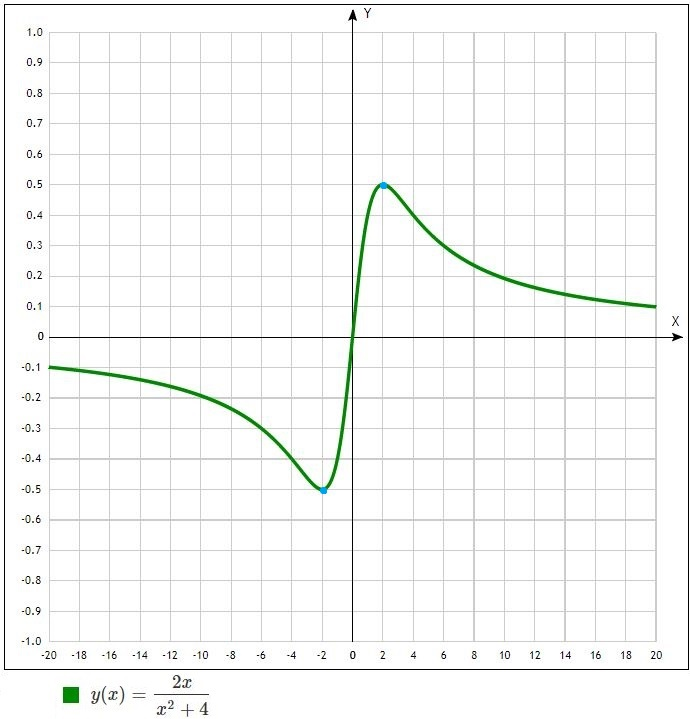
\includegraphics[width=\linewidth]{sol25}\end{figure}\end{minipage}
\end{minipage}\vspace{-5mm}}
{См. график.}{Выполнить все действия по схеме полного исследования функции.}
\end{problem}

\begin{problem}{Построение графиков не типичных функций.}{10.5.12}{10A}{(лёгкая)}
{Провести полное исследование функции $y(x) = \displaystyle \sqrt[3]{1 - x^3}$, нарисовать её график.}
{Функция $y(x)$ определена и непрерывна на всей числовой прямой\\ (корень нечётной степени определён и для положительных, и для отрицательных чисел), поэтому область определения $D(y) = \mathbb{R}$.\smallskip\\
Функция $y(x)$ не является ни чётной, ни нечётной.\smallskip\\
Точек разрыва у $y(x)$ нет, а значит нет и вертикальных асимптот.\smallskip\\
Очевидно, что точка пересечения у $y(x)$ с осью абсцисс только одна~--- это $x = 1$ ($\sqrt[3]{1 - x^3} = 0 \;\Rightarrow\; 1 - x^3 = 0 \;\Rightarrow\; x^3 = 1 \;\Rightarrow\; x = 1$)\smallskip\\
Согласно здравому смыслу, $y(x) > 0$ при $x \in (-\infty; 1)$ и $y(x) < 0$ при $x \in (1; +\infty)$.\smallskip\\
Найдем критические точки функции $y(x)$, решив уравнение $y'(x) = 0$:\\ $\displaystyle y'(x) = \left(\!\sqrt[3]{1 - x^3}\right)' = \frac{-3x^2}{3\sqrt[3]{(1 - x^3)^2}} = -\frac{x^2}{\sqrt[3]{(1 - x^3)^2}} = 0\;\Rightarrow\; x = 0$.\smallskip\\
Теперь найдём промежутки возрастания и убывания:\\ $\displaystyle y'(x) = -\frac{x^2}{\sqrt[3]{(1 - x^3)^2}}$, поэтому согласно методу интервалов, $y(x)$ убывает на $(-\infty; 0) \cup (0; +\infty)$ ($y'(x) < 0$). Отметим, что производная не определена в $x = 1$, но там функция $y(x)$ тоже убывает, просто касательная к графику вертикальна.\smallskip\\
Таким образом, $y(x)$ имеет одну критическую точку, $x = 1$. Однако, поскольку функция всюду убывает, это не точка максимума/минимума, а точка перегиба. Локальных минимумов или максимумов у данной функции $y(x)$ нет.\vspace{-4mm}\\
\begin{minipage}{\linewidth}
    \begin{minipage}{0.4\linewidth}
    \vspace{4mm}
Проверим наличие горизонтальных/наклонных асимптот у функции $y(x)$. Находим $k$:\\ $k = \displaystyle \!\!\lim\limits_{x\to\pm\infty}\!\!\frac{y(x)}{x} = \!\!\lim\limits_{x\to\pm\infty}\!\frac{\sqrt[3]{1 - x^3}}{x} = \lim\limits_{x\to\pm\infty}\!\sqrt[3]{\frac{1 - x^3}{x^3}} = \lim\limits_{x\to\pm\infty}\!\sqrt[3]{\frac{1}{x^3} - 1}$\\ $= \sqrt[3]{0 - 1} = -1$.\medskip\\ Теперь $b$: $\,\displaystyle b = \!\lim\limits_{x\to\pm\infty}(g(x) - kx) = $\\ $\displaystyle = \lim\limits_{x\to\pm\infty}\!\left(\!\sqrt[3]{1 - x^3} + x\!\right) = 0$.\smallskip\\ Следовательно, прямая $y = -x$ является наклонной асимптотой для графика функции $y(x)$.\bigskip\\
График функции $y(x) = \sqrt[3]{1 \!-\! x^3}$ изображён на рисунке справа:
    \end{minipage}
    \hspace{0.02\linewidth}
    \begin{minipage}{0.58\linewidth}\begin{figure}[H] 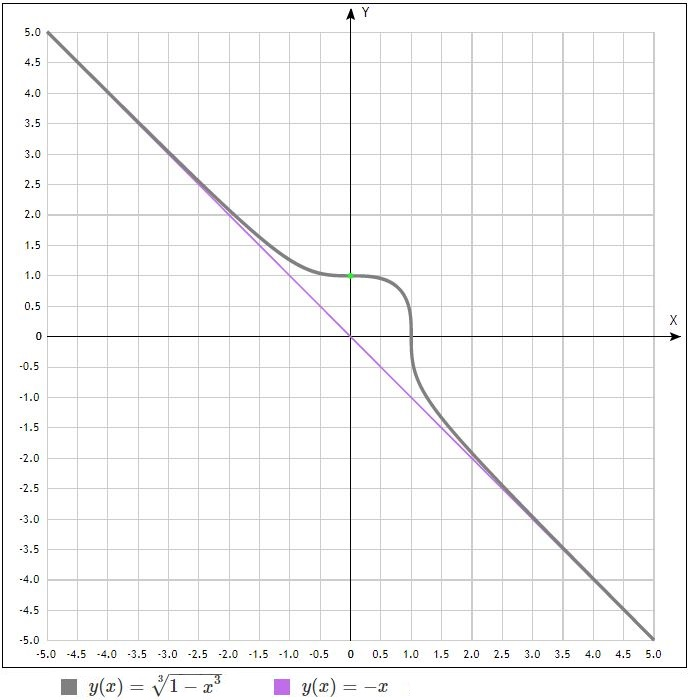
\includegraphics[width=\linewidth]{sol27}\end{figure}\end{minipage}
\end{minipage}\vspace{-1mm}}
{См. график.}{Выполнить все действия по схеме полного исследования функции.}
\end{problem}

\begin{problem}{Применение производной для решения оптимизационных задач.}{10.5.13}{X}{(лёгкая)}
{Зависимость объёма спроса $q$ на продукцию предприятия от цены $p$ (тыс. руб.) задаётся формулой $q = 70 - 5p$. Выручка предприятия за месяц $r$ (тыс. руб.) вычисляется по формуле $r = q \cdot p$. Определить наибольшую цену $p$, при которой выручка составит не менее 240 тыс. руб.}
{НаписанноеРешение}
{ВерныйОтвет}{Подсказка}
\end{problem}

\begin{problem}{Применение производной для решения оптимизационных задач.}{10.5.13}{10A}{(лёгкая)}
{В чебуречной число продаваемых за день чебуреков зависит от цены $p$ (в руб.) и равно $q(p) = 280 - 2p$. Какова выручка чебуречной за день при фиксированной цене чебурека (выручка есть общая величина полученных чебуречной денег). Напиши функцию от $p$. При какой цене чебуреков выручка максимальна?}
{Выручка чебуречной за день равна произведению цены одного чебурека на количество проданных за день чебуреков, то есть $r(p) = p \cdot q(p) = 280p - 2p^2$.\\
Найдём максимум этого выражения. Первый способ: это парабола с ветвями вниз (старший коэффициент отрицателен) $\; \Rightarrow\; $ максимум достигается в вершине параболы, координата которой равна $p_{\text{в}} = -\frac{b}{2a} = -\frac{280}{-4} = 70$. То есть максимальная выручка будет в том случае, если один чебурек стоит 70 рублей.\smallskip\\
Второй способ. Найдём производную $r(p)$: $r'(p) = 280 - 4p$. В критической точке, в том числе и в точке максимума, производная равна 0, откуда $280 - 4p = 0 \;\Rightarrow\; p = \frac{280}{4} = 70$. Проверим, что это действительно максимум: вторая производная $r''(p) = -4 < 0$, а значит это точка максимума, а не минимума (перед точкой $p = 70$ $\,r(p)$ возрастает, а после~--- убывает).}
{Выручка $r = 280p - 2p^2$ максимальна, если один чебурек стоит 70 рублей.}{Выручка равна произведению цены чебурека на число проданных чебуреков. Максимум можно найти либо найдя вершину параболы, либо вычислив производную и решив уравнение для поиска критических точек.}
\end{problem}

\begin{problem}{Применение производной для решения оптимизационных задач.}{10.5.13}{10A}{(лёгкая)}
{Дана функция $f(x) = x^{2}$. Сколько у неё особых точек? Чему равна вторая производная в особых точках? Есть ли у неё минимум / максимум?}
{НаписанноеРешение}
{ВерныйОтвет}{Подсказка}
\end{problem}

\begin{problem}{Применение производной для решения оптимизационных задач.}{10.5.13}{10A}{(лёгкая)}
{Дана функция $f(x) = -x^{2}$. Сколько у неё особых точек? Чему равна вторая производная в особых точках? Есть ли у неё минимум / максимум?}
{НаписанноеРешение}
{ВерныйОтвет}{Подсказка}
\end{problem}

\begin{problem}{Применение производной для решения оптимизационных задач.}{10.5.13}{10A}{(лёгкая)}
{Дана функция $f(x) = x^{3}$. Сколько у неё особых точек? Чему равна вторая производная в особых точках? Есть ли у неё минимум / максимум?}
{По определению, особая точка~--- такая, в которой производная равна 0. Вычислим производную: $f'(x) = 3x^2$. $f'(x) = 0 \;\Rightarrow\; 3x^2 = 0 \;\Rightarrow\; x = 0$, других особых точек нет. Вторая производная равна $6x$ и в этой точке также равна 0.\smallskip\\ Как мы знаем, для наличия максимума в точке $x_0$ требуется выполнение условий $f'(x_0) = 0$ и $f''(x_0) < 0$, а для минимума~--- $f'(x_0) = 0$ и $f''(x_0) > 0$. Следовательно, у данной функции нет ни максимума, ни минимума, а данная точка является точкой перегиба~--- достаточно вспомнить, как выглядит график функции $y = x^3$.}
{Функция $f(x) = x^3$ имеет одну особую точку $x = 0$, однако эта точка является точкой перегиба, а не точкой максимума/минимума.\\ Отмечу, что в этой точке функция <<не растёт>>: касательная к графику является горизонтальной прямой, однако при этом, согласно определению, функция $x^3$ монотонно растёт на всей области определения...}{Каким условиям должна удовлетворять вторая производная функции $f(x)$ для наличия минимума/максимума?}
\end{problem}

\begin{problem}{Применение производной для решения оптимизационных задач.}{10.5.13}{10A}{(лёгкая)}
{Найти максимум функции $W(s) = s^{3} - s^{4} + 5s^{2}$.}
{НаписанноеРешение}
{ВерныйОтвет}{Подсказка}
\end{problem}

\begin{problem}{Применение производной для решения оптимизационных задач.}{10.5.13}{10A}{(лёгкая)}
{Найти минимум функции $K(x) = x^4 + 4x^3 - 56x^2$.}
{Для нахождения минимума в первую очередь находим критические точки~--- те точки, где $K'(x) = 0$. $K'(x) = 4x^3 + 12x^2 - 112x$.\\ Получаем уравнение третьей степени $4x^3 + 12x^2 - 112x = 0$.\\ Решаем: $4x^3 + 12x^2 - 112x = 0 \;\Rightarrow\; x(x^2 + 3x - 28) = 0 \;\Rightarrow\; x(x - 4)(x + 7) = 0$.\\ Таким  образом, есть три критические точки, $x = -7$, $x = 0$ и $x = 4$.\\
Для того, чтобы критическая точка $x_0$ была точкой минимума, должно быть выполнено неравенство $K''(x_0) > 0$. Находим вторую производную: $K''(x) = (4x^3 + 12x^2 - 112x)' = 12x^2 + 24x - 112 = 4(3x^2 + 8x - 28) = 4(x - 2)(3x + 14)$.\\ В точках $x = -7$ и $x = 4$ вторая производная положительна, в точке $x = 0$ вторая производная отрицательна. Таким образом, $x = -7$ и $x = 4$~--- точки локальных минимумов. Глобальный минимум достигается в точке $x = -7$, поскольку $(-7)^4 + 4\cdot (-7)^3 - 56\cdot(-7)^2 < 4^4 + 4^4 - 56\cdot4^2$. $\,K(-7) = (7 - 4 - 8)\cdot7^3 = -1715$.}
{Данная функция имеет два локальных минимума, при $x = -7$ и $x = 4$. Глобальный минимум достигается при $x = -7\,$ и $\,K(-7) = -1715$.}{Какому условию должна удовлетворять вторая производная $K''(x_0)$ для того, чтобы $K$ имела минимум в точке $x_0$?}
\end{problem}

\begin{problem}{Применение производной для решения оптимизационных задач.}{10.5.13}{10A}{(лёгкая)}
{Исследовать функцию $G(t) = t^4 - 4t^3$ на минимумы и максимумы.}
{Для нахождения локальных экстремумов в первую очередь находим критические точки~--- точки, где $G'(t) = 0$. $\,G'(t) = 4t^3 - 12t^2$.\\ Получаем уравнение: $\,4t^3 - 12t^2 = 0 \;\Rightarrow\; 4t^2(t - 3) = 0 \;\Rightarrow\; t = 0$, $\,t = 3$.\\
Находим вторую производную и её значение в полученных критических точках:\\ $G''(t) = 12t^2 - 24t \;\Rightarrow\; G''(0) = 0$, $\,G''(3) = 108 - 72 = 36 > 0$. Таким образом, точка $t = 0$~--- точка перегиба, а точка $t = 3$~--- точка локального минимума.\\ Глобального и локального максимума нет: функция $G(t)$ неограниченно возрастает при $t \to -\infty$ и $t \to \infty$.}
{У функции $G(t)$ есть только один минимум в точке $t = 3$, максимума нет.}{Найти все особые точки функции $G(t)$ и вычислить в них знаки второй производной.}
\end{problem}

\begin{problem}{Применение производной для решения оптимизационных задач.}{10.5.13}{10A}{*}
{Для функции $T(x) = -3x^2 + \frac{17}{3}x^3 - \frac{11}{4}x^4 - 2x^5 + \frac{8}{3}x^6 - x^7 + \frac{1}{8}x^8$ найти все локальные минимумы и максимумы. Нарисовать примерный график.}
{Как обычно, в первую очередь находим особые точки, которые удовлетворяют условию первого порядка $T'(x) = 0$.\\ Получаем следующее уравнение: $\,-6x + 17x^2 - 11x^3 - 10x^4 + 16x^5 - 7x^6 + x^7 = 0$\\
$\;\Rightarrow\; x(x^6 - 7x^5 + 16x^4 - 10x^3 - 11x^2 + 17x - 6) = 0$.\\ Можно угадать корень: сумма коэффициентов равна 0, поэтому $x = 1$ является корнем. Раскладываем на множители (выносим $x - 1$), получаем, что\\
$x(x - 1)(x^5 - 6x^4 + 10x^3 - 11x + 6) = 0$. Повторяем то же самое, так как сумма коэффициентов снова равна 0 $\;\Rightarrow\; x(x - 1)^2(x^4 - 5x^3 + 5x^2 + 5x - 6) = 0$.\\ И неожиданно, снова сумма коэффициентов равна 0, поэтому снова выносим $(x - 1)$: приходим к уравнению $x(x - 1)^3(x^3 - 4x^2 + x + 6) = 0$. У полученного выражения $x^3 - 4x^2 + x + 6$ сумма коэффициентов не равна нулю, но равна нулю знакопеременная сумма коэффициентов (сумма коэффициентов, стоящих при чётных степенях, равна сумме коэффициентов, стоящих при нечётных).\\ Поэтому $x = -1$ является корнем и можно вынести множитель $x + 1$:\\
$x^3 - 4x^2 + x + 6 = (x + 1)(x^2 - 5x + 6)$. Квадратное уравнение $x^2 - 5x + 6 = 0$ решаем через дискриминант: $D = 25 - 24 = 1 \;\Rightarrow\; x_{1,2} = \frac{5\pm1}{2} = 2; 3$.\smallskip\\
Итого: $T'(x) = -6x + 17x^2 - 11x^3 - 10x^4 + 16x^5 - 7x^6 + x^7 = x(x + 1)(x - 1)^3(x -\\- 2)(x - 3) = 0$ и функция $T(x)$ имеет 5 особых точек: $x = -1; \,0;\, 1;\, 2;\, 3$.\\
\vspace{-8mm}\\\begin{minipage}{\linewidth}
    \begin{minipage}{0.48\linewidth}
    Для того, чтобы отличить минимумы от максимумов, используем хитрость:\smallskip\\ $T'(x) = x(x + 1)(x - 1)^3(x - 2)(x - 3) \;\Rightarrow\;$ согласно методу интервалов $T'(x) < 0$ при $x \in (-\infty; -1) \cup (0; 1) \cup (2; 3)$ и \\(тоже по методу интервалов) $T'(x) > 0$\\ при $x \in (-1; 0) \cup (1; 2) \cup (3; +\infty)$.\medskip\\ Значит, поскольку перед особыми точками $x = -1$, $x = 1$, $x = 3$ производная отрицательна, эти точки должны быть точками минимума, а точки $x = 0$ и $x = 2$~--- точками максимума.\smallskip\\
    График функции $T(x)$ изображён на рисунке справа.
    \end{minipage}
    \hspace{0.02\linewidth}
    \begin{minipage}{0.49\linewidth}\begin{figure}[H] 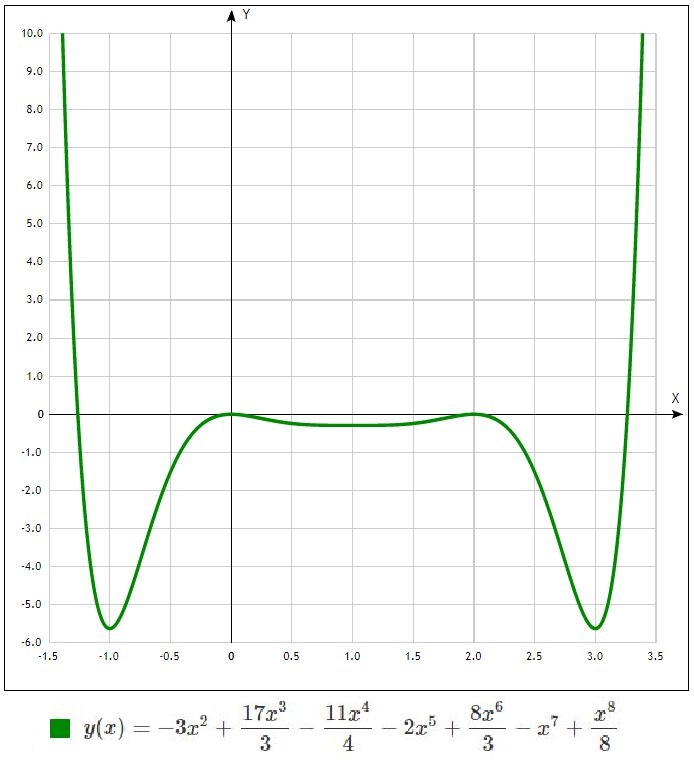
\includegraphics[width=\linewidth]{sol15}\end{figure}\end{minipage}
\end{minipage}}
{Функция $T(x)$ имеет локальные минимумы при $x = -1$, $x = 1$, $x = 3$, и локальные максимумы при $x = 0$ и $x = 2$.}{Получаемое при нахождении особых точек уравнение высокого порядка на самом деле имеет целые корни~--- что позволяет его решить с помощью теоремы Безу.}
\end{problem}

\begin{problem}{Применение производной для решения оптимизационных задач.}{10.1.13}{10A}{*}
{Произведение двух положительных чисел равно 324.\\ Чему равно наименьшее значение суммы этих двух чисел?}
{Пусть $a$~--- первое число, $b$~--- второе число. Тогда $ab = 324$, а мы хотим решить задачу $a + b \to \min$. Чтобы данное выражение, минимум которого мы ищем, было функцией от одной переменной, воспользуемся тем, что мы можем выразить $b$ через $a$: $\,b = \frac{324}{a}$. Таким образом, мы решаем задачу $a + \frac{324}{a} \to \min$.\smallskip\\
Данное выражение достигает минимума в неизвестной нам точке, но мы точно знаем, что в точке минимума производная будет равна 0, поэтому вычислим производную: $\;\left(a + \frac{324}{a}\right)' = a' + 324\cdot\left(\frac{1}{a}\right)' = 1 + 324\cdot\left(-\frac{1}{a^2}\right) = 1 - \frac{324}{a^2}$.\smallskip\\ Производная должна быть равна 0: $1 - \frac{324}{a^2} = 0 \Rightarrow 1 = \frac{324}{a^2} \Rightarrow a^2 = 324 \Rightarrow a \pm 18.$\\
У нас есть две точки, где достигается то ли максимум, то ли минимум, однако по условию оба числа положительны, поэтому $a > 0$ и надо проверить только $a = 18$.\\ В этом случае $b = 324:18 = 18$, и $a + b = 36$. Если $a$ будет близко к нулю, то большим будет $b$, и сумма будет больше 36. Если же $a$ велико, то $b$ и $a$ просто меняются местами, и сумма опять же будет больше 36.\\ Поэтому наименьшая сумма двух чисел равна 36.}
{Наименьшее значение суммы этих двух чисел равно 36.}{Надо выразить одно число через второе, а после этого уже искать минимум функции с помощью производной.}
\end{problem}

\begin{problem}{Применение производной для решения оптимизационных задач.}{10.5.13}{10A мб плохо, так как есть цилиндр}{(лёгкая)}
{Магазин ГлавРыба продаёт кильку в томате, в консервных банках цилиндрической формы (с фиксированными $r$ и $h$). Каковы должны быть размеры этих консервных банок, чтобы на их изготовление шло наименьшее количество материала, при том что объём банки составляет неизменные $0{,}25$ литра?\\
{\slshape Комментарий:} $\,V_{\text{цилиндра}} = \pi r^2 \cdot h$, $\,S_{\text{поверхности цилиндра}} = 2\cdot\pi r^2 + h\cdot 2\pi r$. }
{Составим уравнение: объём цилидрической банки равен $\pi r^2\cdot h$.\\ Отсюда $\pi r^2 h = 250$ см$^3$. Количество материала равно площади всей поверхности: площадь оснований равна $2\cdot\pi r^2$, а площадь боковой поверхности равна $h\cdot 2\pi r$.\smallskip\\ Таким образом, мы решаем задачу $2\pi r^2 + 2\pi rh \to \min$.\\ Используя первое уравнение, выразим $h$ через $r$: $\,h = \frac{250}{\pi r^2}$. Подставляем:\smallskip\\
\hspace*{3cm}$\displaystyle 2\pi r^2 + 2\pi r\cdot \frac{250}{\pi r^2} \to \min$, то есть $\,\displaystyle 2\pi r^2 + \frac{500}{r} \to \min$.\smallskip\\
Исследуем функцию $S(r) = 2\pi r^2 + \frac{500}{r}$ c помощью производной: минимум $S(r)$ может достигаться только тогда, когда производная $S$ равна нулю, поэтому вычислим $S'(r)$ и приравняем полученное значение к нулю:\smallskip\\
$S'(r) = \left(2\pi r^2 + \frac{500}{r}\right)' = 2\pi \cdot 2r + 500 \cdot \left(-\frac{1}{r^2}\right) = 4\pi r - \frac{500}{r^2} = 0$. Решаем полученное рациональное уравнение: $4\pi r - \frac{500}{r^2} = 0 \;\Rightarrow\; 4\pi r = \frac{500}{r^2} \;\Rightarrow\; 4\pi r^3 = 500 \;\Rightarrow\; r = \frac{5}{\sqrt[3]{\pi}}$. Получаем, что $h$ равно $\,\displaystyle \frac{250}{\pi r^2} = \frac{250}{\pi\cdot \left(\frac{5}{\sqrt[3]{\pi}}\right)^{\!2}} = \frac{10}{\sqrt[3]{\pi}}$. $\;$ Итого: $r = \frac{5}{\sqrt[3]{\pi}}$, $\,h = \frac{10}{\sqrt[3]{\pi}}$.\\
Интуитивно понятно, что в этом случае площадь наименьшая, а не наибольшая, так что это и есть ответ.}
{У <<оптимальной>> банки $r = \frac{5}{\sqrt[3]{\pi}} \approx 3{,}4$ см, $\,h = \frac{10}{\sqrt[3]{\pi}} \approx 6{,}8$ см.\smallskip\\ Отмечу, что отсюда следует легко запоминающийся вывод: наименьшая площадь поверхности у цилиндра будет в том случае, если его высота равна его диаметру.\\ (И поэтому классическая советская банка сгущёнки имеет квадратный профиль)}{Надо выразить $h$ через $r$ и затем использовать производную.}
\end{problem}

\begin{problem}{Применение производной для решения оптимизационных задач.}{10.5.13}{10A}{*}
{Чему равно наименьшее значение $k = \frac{V_\text{к}}{V_\text{ц}}$, где $V_\text{к}$ и $V_\text{ц}$~--- объёмы конуса и цилиндра, описанных около одной сферы?}
{Для начала определимся с цилиндром: очевидно, что его радиус будет равен радиусу сферы $r$, а его высота будет равна $2r$. Поэтому объём цилиндра $V_\text{ц}$ равен $\pi r^2 \cdot 2r = 2\pi r^3$. Теперь конус. Нам неизвестны ни его радиус, ни его высота.
\vspace{-6mm}\\\begin{minipage}{\linewidth}
    \begin{minipage}{0.58\linewidth}
    Проведём осевое сечение: получится треугольник $ABC$, изображённый на рисунке справа.\smallskip\\ Здесь $R$ --- радиус конуса, $h$ --- его высота, $O$ --- центр нашей сферы радиуса $r$, точки $D$, $E$, $H$ --- точки касания сферы с конусом (и поэтому в этих точках радиусы образуют с касательными прямые углы). Согласно формуле для объёма конуса, $V_\text{к} = \frac13Sh = \frac13\pi R^2h$.\medskip\\ Выясним, как связаны между собой $R$, $h$, $r$, и $x$ (отрезок $AD$). В силу подобия треугольников $AOD$ и $ABH$, отношение катетов постоянно: $\frac{r}{x} = \frac{R}{h}$. Вдобавок к этому, как и в любом прямоугольном треугольнике, выполнена теорема Пифагора: для треугольника $AOD$ имеем $(h-r)^2 = x^2 + r^2$, откуда $x^2 = h^2 - 2hr$.
    \end{minipage}
    \hspace{0.01\linewidth}
    \begin{minipage}{0.4\linewidth}\begin{figure}[H] 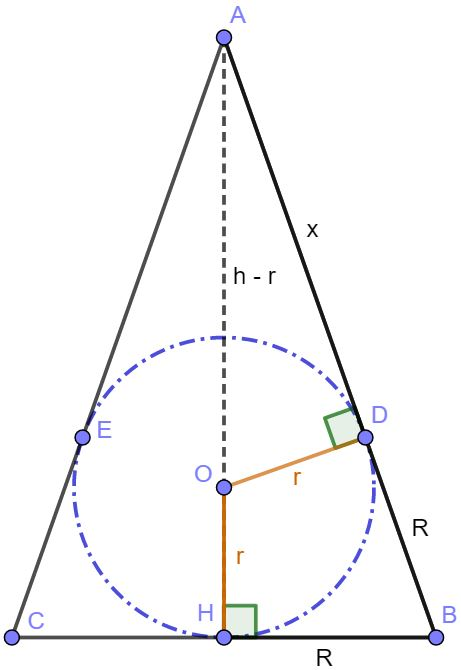
\includegraphics[width=\linewidth]{sol67}\end{figure}\end{minipage}
\end{minipage}
Какую задачу нам надо решить? Мы хотим решить оптимизационную задачу $\displaystyle k = \frac{V_\text{к}}{V_\text{ц}} \to \min$, или, в наших обозначениях, $\displaystyle \frac{\frac13\pi R^2h}{2\pi r^3} \to \min$. Немного упростим: $\displaystyle \frac{R^2h}{6r^3} \to \min$, что то же самое, что и $\displaystyle \frac{R^2h}{r^3} \to \min$. Мы умеем находить минимумы функций, в том случае, если переменная всего одна. Осталось этого добиться. $\frac rx = \frac Rh \Rightarrow R^2 = \frac{r^2h^2}{x^2} = \frac{r^2h^2}{h^2 - 2hr} \;\Rightarrow\; \frac{r^2h^2}{h^2 - 2hr}\cdot\frac{h}{r^3} \to \min \;\Rightarrow\; \frac{h^2}{rh - 2r^2} \to \min$.\\
Мы использовали оба доступных нам уравнения, а в нашем выражении всё ещё осталось две неизвестных, а не одна. Но от величины $r$ ничего не зависит, это просто выбор масштаба. То есть функция $k(h, r) = \frac{h^2}{rh - 2r^2}$ является однородной: $k(ch, cr) = k(h, r)$. Используем стандартный приём: $k = \frac{h^2}{rh - 2r^2} = \frac{\frac{h^2}{r^2}}{\frac hr - 2} = \frac{t^2}{t - 2}$.\\
Находим минимум данной функции по $t$: $\;k'(t) = \frac{2t(t-2) - t^2}{(t - 2)^2} = \frac{t(t - 4)}{(t - 2)^2} = 0$.\\ После проверки можно убедиться, что точка $t = 0$ даёт локальный максимум, а $\,t = 4$ --- минимум. Значит, $\frac hr = 4 \;\Rightarrow\; h = 4r \;\Rightarrow\; k_{\text{min}} = \frac{(4r)^2}{6\cdot(r\cdot4r - 2r^2)} = \frac{16}{12} = \frac43$.}
{Искомое наименьшее значение $k$ равно $\frac43$.}{Найти $V_\text{ц}(r)$. Рассмотреть осевое сечение конуса и связать $r$, $h$, $R$. Получить выражение для $k(r, h)$ и заметить, что это однородная функция (то есть отношение объёмов не меняется, если просто изменить масштаб).\\ С помощью стандартного метода, используемого для решения однородных уравнений, свести задачу к поиску минимума функции одной переменной $k(t) \to \min$.}
\end{problem}

\begin{problem}{Применение производной для решения оптимизационных задач.}{10.5.13}{10A}{(лёгкая)}
{Из куска проволоки длиной 50 см требуется согнуть прямоугольник наибольшей площади. Каковы размеры этого прямоугольника?}
{НаписанноеРешение}
{ВерныйОтвет}{Подсказка}
\end{problem}

\begin{problem}{Применение производной для решения оптимизационных задач.}{10.1.13}{10A red сделать рисунок}{(лёгкая)}
{Из прямоугольного листа картона со сторонами 30 и 80 сантиметров вырезают коробку: от каждого уголка отрезают квадрат со стороной $x$, а затем полученный <<крест>> складывают и склеивают скотчем. Какого размера квадрат надо отрезать, чтобы объём полученной коробки был наибольшим?}
{После вырезания квадрата со стороной $x$, стороны получившейся коробки будут равны $x$, $30 - 2x$, и $80 - 2x$ (смотри рисунок ниже).
\vspace{-4mm}\\\begin{minipage}{\linewidth}
    \begin{minipage}{0.36\linewidth}
    То есть объём коробки является функцией от $x$ и равен $V(x) = x(30 - 2x)(80 - 2x) = 4x^3 - 220x^2 + 2400x$.
    \end{minipage}
    \hspace{0.03\linewidth}
    \begin{minipage}{0.6\linewidth}\begin{figure}[H] 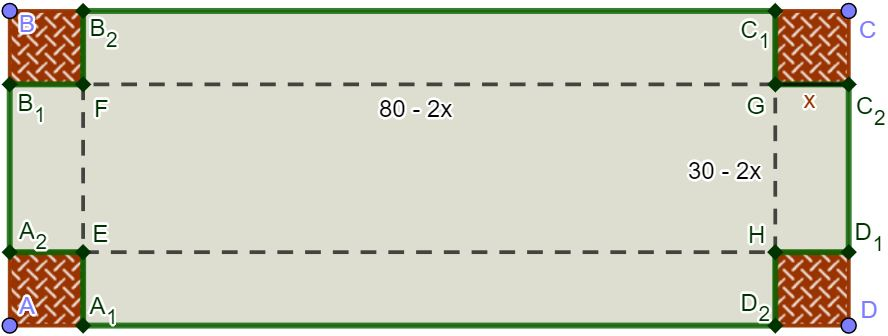
\includegraphics[width=\linewidth]{sol59}\end{figure}\end{minipage}\smallskip
\end{minipage}
Мы хотим найти максимум $V(x)$. Это кубическая функция с положительным старшим коэффициентом, мы знаем, что при $x \to \infty$ она безгранично растёт. Однако, нас интересует максимум на отрезке $[0; 15]$, так как сторона отрезаемого квадрата не может быть отрицательна или больше 15 сантиметров.\\ Проверим значения на концах отрезка: $V(0) = 0$ (ничего не отрезали, коробка плоская), $V(15) = 0$ (отрезали так, что от ширины ничего не осталось).\\ Поэтому нужный нам максимум находится где-то внутри отрезка, и для него верно $V'(x) = 0$ (когда объём достигает максимума, функция не растёт и не убывает).\smallskip\\
Найдём производную $V'(x)$: для этого используем следующие правила дифференцирования: $(f + g)' = f' + g'$; $\quad(Cf)' = C\cdot f'$; $\quad(x^n)' = nx^{n - 1}$.\smallskip\\
$V'(x) = (4x^3 - 220x^2 + 2400x)' = (4x^3)' - (220x^2)' + (2400x)' = 4(x^3)' - 220(x^2)' + 2400(x)' = 4\cdot3x^2 - 220\cdot2x + 2400\cdot1 = 12x^2 - 440x + 2400 = 0$.\\
Решаем полученное квадратное уравнение на $x$: $\,12x^2 - 440x + 2400 = 0 \;\Rightarrow\; 3x^2 - 110x + 600 = 0 \;\Rightarrow\; D = 110^2 - 12\cdot600 = 100\cdot(121 - 72) = 4900$.\\
$\Rightarrow\; x = \frac{110\pm70}{6} = 30; \,\frac{20}{3}$. Первое значение находится не в интересующем нас интервале, а вот второе как раз в нём. Проверим, что это максимум, а не минимум: $V\!\left(\frac{20}{3}\right) = \frac{20}{3}\cdot\frac{50}{3}\cdot\frac{200}{3} = \frac{200000}{27}$, что больше, чем значения на концах нашего отрезка.

}
{Объём коробки будет максимальным, если взять $x = \frac{20}{3}$ (то есть надо отрезать квадрат со стороной $7\frac13$ сантиметра).}{Нужно представить объём коробки как функцию от $x$, и найти\\ максимальное значение этого объёма, используя производную ($V'(x) = 0$).}
\end{problem}

\begin{problem}{Применение производной для решения оптимизационных задач.}{10.1.13}{10A}{(лёгкая)}
{В арифметической прогрессии шестой член равен 3, а разность прогрессии больше $0{,}5$. При каком значении разности этой прогрессии произведение первого, четвёртого, и пятого её членов является наибольшим?}
{Как нам известно, арифметическая прогрессия полностью определяется $a = x_1$~--- значением первого члена прогрессии и $d$~--- разностью прогрессии. Мы знаем, что $a + 5d = 3$, откуда $a = 3 - 5d$, а также что $d > 0{,}5$.\\ Сформулируем, какую задачу нам нужно решить: мы хотим максимизировать произведение трёх членов прогрессии, то есть $x_1 \cdot x_4 \cdot x_5 \to \max$, или, что то же самое, $a \cdot (a + 3d) \cdot (a + 4d) \to \max$.\\ С учётом уравнения $a = 3 - 5d$, получаем задачу, которую мы умеем решать: $(3 - 5d) \cdot (3 - 2d) \cdot (3 - d) \to \max$, поиск максимума функции одной переменной.\smallskip\\
Итак, мы исследуем функцию $p(d) = (3 - 5d) \cdot (3 - 2d) \cdot (3 - d)$. Раскроем скобки и запишем получившийся многочлен 3 степени в стандартном виде: получаем, что $p(d) = -10d^3 + 51d^2 - 72d + 27$. Находим производную: $p'(d) = -30d^2 + 102d - 72$.\smallskip\\
Для нахождения критических точек приравниваем производную к нулю и решаем квадратное уравнение: $-30d^2 + 102d - 72 = 0 \;\Rightarrow\; -3 \cdot (10d^2 - 34d + 24) = -3 \cdot (d - 1)(10d - 24) = 0$. Таким образом, мы находим две критические точки $d = 1$ и $d = 2{,}4$. Однако, стоит вспомнить, что мы ищем максимум на луче!\\ В самом деле, так как $d > 0{,}5$, мы ищем максимум на интервале $(\frac12; +\infty)$.\smallskip\\ На интервале $(\frac12;\, 1)$, согласно методу интервалов, $p(d)$ убывает ($p'(d) < 0$).\\ На интервале $(1; \,2{,}4)$ $p(d)$ возрастает, а на интервале $(2{,}4;\, +\infty)$~--- опять убывает.\\
Поскольку $p(d)$~--- многочлен 3 степени, это непрерывная функция, точек разрыва нет. Поэтому в точке $d = 2{,}4$ достигается локальный максимум, и получающееся произведение равно $p(2{,}4) = \frac{243}{25} = 9{,}72$. Проверим также точку $d = \frac12$: $p\left(\frac12\right) = (3 - \frac52)(3 - 1)(3 - \frac12) = \frac52 < p(2{,}4)$. Следовательно, разность равна $2{,}4$.}
{Произведение этих трёх членов прогрессии будет наибольшим, если из всех возможных $d$ ($d > 0{,}5$) выбрать $d = 2{,}4$.}{Арифметическая прогрессия определяется двумя числами.\\ Первое условие позволяет выразить одно через другое и далее решать обычную оптимизационную задачу. Второе условие позволяет сузить область поиска.}
\end{problem}

\begin{problem}{Применение производной для решения оптимизационных задач.}{10.5.13}{10A}{*}
{В полукруг радиуса 15 вписан прямоугольник наибольшего возможного периметра. Чему равен этот периметр?}
{Сначала разберёмся, как именно вписан прямоугольник: после изучения картинки становится понятно, что прямоугольник <<лежит>> на диаметре этого полукруга, а другие две точки касаются полуокружности.
\vspace{-4mm}\\\begin{minipage}{\linewidth}
    \begin{minipage}{0.41\linewidth}
    ~\vspace{1mm}\\
    Это означает, что если ширина этого прямоугольника равна $x$, то по теореме Пифагора половина его длины равна $\frac{y}{2} = \sqrt{15^2 - x^2}$.\smallskip\\
    Таким образом, длина прямоугольника $y = 2\sqrt{225 - x^2}$, и периметр зависит от ширины $x$ как\vspace{-3mm} $$P(x) = 2x + 4\sqrt{225 - x^2}.$$
    \end{minipage}
    \hspace{0.02\linewidth}
    \begin{minipage}{0.57\linewidth}\begin{figure}[H] 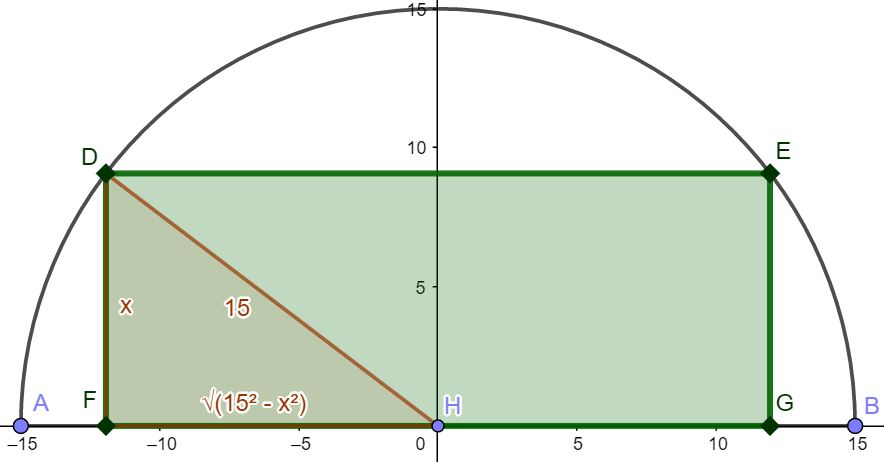
\includegraphics[width=\linewidth]{sol61}\end{figure}\end{minipage}\medskip
\end{minipage}
Значит, наша задача~--- найти максимум этой функции. Находим производную, приравниваем к нулю: $P'(x) = 2 + \frac{4}{2\sqrt{225 - x^2}}\cdot(-2x) = 2 - \frac{4x}{\sqrt{225 - x^2}}$.\\
$2 - \frac{4x}{\sqrt{225 - x^2}} = 0 \;\Rightarrow\; 2 = \frac{4x}{\sqrt{225 - x^2}} \;\Rightarrow\; 4 = \frac{16x^2}{225 - x^2} \;\Rightarrow\; 900 - 4x^2 = 16x^2 \;\Rightarrow\; 45 = x^2$.\smallskip\\
Отсюда получаем, что $x = 3\sqrt{5}$ (ширина не может быть отрицательной).\\ Находим длину: $y = 2\sqrt{225 - 45} = 2\sqrt{180} = 6\sqrt{20} = 12\sqrt{5}$.\\ Следовательно, периметр будет равен $30\sqrt{5} \approx 67$ сантиметров.}
{Этот периметр равен $30\sqrt{5}$ см и достигается в том случае, если ширина равна $3\sqrt{5}$ см, а длина~--- $12\sqrt{5}$ см.}{Пусть ширина прямоугольника равна $x$. Чему тогда равна половина его длины? Составить выражение $P(x)$ и решить задачу $P(x) \to \max$.}
\end{problem}

\end{document}